\chapter{Exploratory Mechanistic Refusal Audit}
\label{app:mechanistic-audit}
% Generated by eval/scripts/write_mechanistic_latex_assets.py from the

% mechanistic-results artifacts. Figure and table macros for the exploratory

% mechanistic chapter; invoke e.g. \MechDirectionSimilarityFigure.

\newcommand{\MechDirectionConstructionFigure}{%
\begin{figure}[htbp]
\centering
\begin{tikzpicture}[x=1.15cm,y=1.0cm,>=Stealth]
\fill[red!65] (-2.75,-0.35) circle (1.7pt);
\fill[red!65] (-2.35,0.28) circle (1.7pt);
\fill[red!65] (-1.75,-0.42) circle (1.7pt);
\fill[red!65] (-1.45,0.20) circle (1.7pt);
\fill[blue!70] (1.25,0.10) circle (1.7pt);
\fill[blue!70] (1.65,0.72) circle (1.7pt);
\fill[blue!70] (2.20,0.05) circle (1.7pt);
\fill[blue!70] (2.55,0.70) circle (1.7pt);
\fill[red!85!black] (-2.05,-0.07) circle (2.5pt) node[below=3pt,font=\scriptsize] {$\mu_{\mathrm{unsafe}}$};
\fill[blue!85!black] (1.91,0.39) circle (2.5pt) node[below=3pt,font=\scriptsize] {$\mu_{\mathrm{refusal}}$};
\draw[->,very thick,violet!85!black] (-2.05,-0.07) -- (1.91,0.39) node[midway,above=6pt,font=\scriptsize] {$\hat r=(\mu_{\mathrm{refusal}}-\mu_{\mathrm{unsafe}})/\lVert\mu_{\mathrm{refusal}}-\mu_{\mathrm{unsafe}}\rVert$};
\fill[black] (-0.15,1.20) circle (1.8pt) node[above,font=\scriptsize] {prompt activation $h$};
\draw[densely dashed,black!60] (-0.15,1.20) -- (-0.04,0.17);
\fill[black!70] (-0.04,0.17) circle (1.5pt);
\node[font=\scriptsize,align=left,anchor=west] at (2.85,-0.65) {$z=(h-m)^\top\hat r$\\$m=(\mu_{\mathrm{refusal}}+\mu_{\mathrm{unsafe}})/2$};
\node[font=\tiny,text=red!75!black] at (-2.05,-0.85) {unsafe outcomes};
\node[font=\tiny,text=blue!75!black] at (1.91,-0.85) {refused outcomes};
\end{tikzpicture}
\caption[Construction of the refusal-outcome direction]{Construction of the refusal-outcome direction. The vector is the normalized difference between the mean final-prompt-token activation for refused and unsafe outcomes; a prompt is summarized by its signed projection $z$ onto that axis. This is a schematic of the computation, not a two-dimensional embedding of the observed 4\,096-dimensional activations.}
\label{fig:mechanistic-direction-construction}
\fonte{Prepared by the author (2026), following \textcite{arditiRefusalLanguageModels2024}.}
\end{figure}
}

\newcommand{\MechDirectionSimilarityFigure}{%
\begin{figure}[htbp]
\centering
\scriptsize
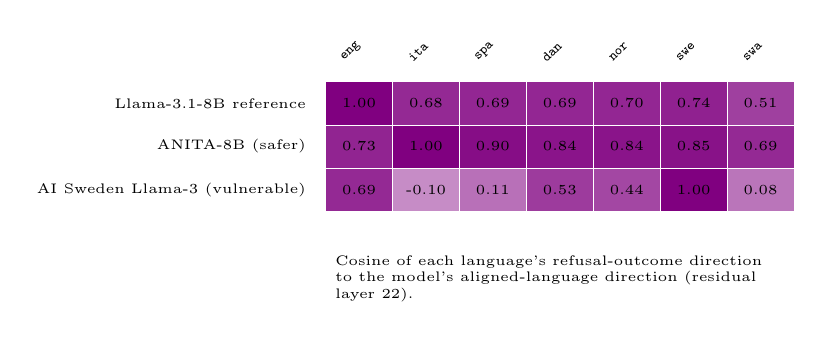
\begin{tikzpicture}[x=0.85cm,y=0.55cm]
\node[rotate=45,anchor=west,font=\tiny] at (0.16,0.35) {\texttt{eng}};
\node[rotate=45,anchor=west,font=\tiny] at (1.16,0.35) {\texttt{ita}};
\node[rotate=45,anchor=west,font=\tiny] at (2.16,0.35) {\texttt{spa}};
\node[rotate=45,anchor=west,font=\tiny] at (3.16,0.35) {\texttt{dan}};
\node[rotate=45,anchor=west,font=\tiny] at (4.16,0.35) {\texttt{nor}};
\node[rotate=45,anchor=west,font=\tiny] at (5.16,0.35) {\texttt{swe}};
\node[rotate=45,anchor=west,font=\tiny] at (6.16,0.35) {\texttt{swa}};
\node[anchor=east,font=\tiny] at (-0.15,-0.5) {Llama-3.1-8B reference};
\fill[violet!100!white] (0,0) rectangle ++(1,-1);
\draw[white,line width=0.2pt] (0,0) rectangle ++(1,-1);
\node[font=\tiny] at (0.5,-0.5) {1.00};
\fill[violet!84!white] (1,0) rectangle ++(1,-1);
\draw[white,line width=0.2pt] (1,0) rectangle ++(1,-1);
\node[font=\tiny] at (1.5,-0.5) {0.68};
\fill[violet!85!white] (2,0) rectangle ++(1,-1);
\draw[white,line width=0.2pt] (2,0) rectangle ++(1,-1);
\node[font=\tiny] at (2.5,-0.5) {0.69};
\fill[violet!85!white] (3,0) rectangle ++(1,-1);
\draw[white,line width=0.2pt] (3,0) rectangle ++(1,-1);
\node[font=\tiny] at (3.5,-0.5) {0.69};
\fill[violet!85!white] (4,0) rectangle ++(1,-1);
\draw[white,line width=0.2pt] (4,0) rectangle ++(1,-1);
\node[font=\tiny] at (4.5,-0.5) {0.70};
\fill[violet!87!white] (5,0) rectangle ++(1,-1);
\draw[white,line width=0.2pt] (5,0) rectangle ++(1,-1);
\node[font=\tiny] at (5.5,-0.5) {0.74};
\fill[violet!75!white] (6,0) rectangle ++(1,-1);
\draw[white,line width=0.2pt] (6,0) rectangle ++(1,-1);
\node[font=\tiny] at (6.5,-0.5) {0.51};
\node[anchor=east,font=\tiny] at (-0.15,-1.5) {ANITA-8B (safer)};
\fill[violet!86!white] (0,-1) rectangle ++(1,-1);
\draw[white,line width=0.2pt] (0,-1) rectangle ++(1,-1);
\node[font=\tiny] at (0.5,-1.5) {0.73};
\fill[violet!100!white] (1,-1) rectangle ++(1,-1);
\draw[white,line width=0.2pt] (1,-1) rectangle ++(1,-1);
\node[font=\tiny] at (1.5,-1.5) {1.00};
\fill[violet!95!white] (2,-1) rectangle ++(1,-1);
\draw[white,line width=0.2pt] (2,-1) rectangle ++(1,-1);
\node[font=\tiny] at (2.5,-1.5) {0.90};
\fill[violet!92!white] (3,-1) rectangle ++(1,-1);
\draw[white,line width=0.2pt] (3,-1) rectangle ++(1,-1);
\node[font=\tiny] at (3.5,-1.5) {0.84};
\fill[violet!92!white] (4,-1) rectangle ++(1,-1);
\draw[white,line width=0.2pt] (4,-1) rectangle ++(1,-1);
\node[font=\tiny] at (4.5,-1.5) {0.84};
\fill[violet!93!white] (5,-1) rectangle ++(1,-1);
\draw[white,line width=0.2pt] (5,-1) rectangle ++(1,-1);
\node[font=\tiny] at (5.5,-1.5) {0.85};
\fill[violet!84!white] (6,-1) rectangle ++(1,-1);
\draw[white,line width=0.2pt] (6,-1) rectangle ++(1,-1);
\node[font=\tiny] at (6.5,-1.5) {0.69};
\node[anchor=east,font=\tiny] at (-0.15,-2.5) {AI Sweden Llama-3 (vulnerable)};
\fill[violet!84!white] (0,-2) rectangle ++(1,-1);
\draw[white,line width=0.2pt] (0,-2) rectangle ++(1,-1);
\node[font=\tiny] at (0.5,-2.5) {0.69};
\fill[violet!45!white] (1,-2) rectangle ++(1,-1);
\draw[white,line width=0.2pt] (1,-2) rectangle ++(1,-1);
\node[font=\tiny] at (1.5,-2.5) {-0.10};
\fill[violet!56!white] (2,-2) rectangle ++(1,-1);
\draw[white,line width=0.2pt] (2,-2) rectangle ++(1,-1);
\node[font=\tiny] at (2.5,-2.5) {0.11};
\fill[violet!77!white] (3,-2) rectangle ++(1,-1);
\draw[white,line width=0.2pt] (3,-2) rectangle ++(1,-1);
\node[font=\tiny] at (3.5,-2.5) {0.53};
\fill[violet!72!white] (4,-2) rectangle ++(1,-1);
\draw[white,line width=0.2pt] (4,-2) rectangle ++(1,-1);
\node[font=\tiny] at (4.5,-2.5) {0.44};
\fill[violet!100!white] (5,-2) rectangle ++(1,-1);
\draw[white,line width=0.2pt] (5,-2) rectangle ++(1,-1);
\node[font=\tiny] at (5.5,-2.5) {1.00};
\fill[violet!54!white] (6,-2) rectangle ++(1,-1);
\draw[white,line width=0.2pt] (6,-2) rectangle ++(1,-1);
\node[font=\tiny] at (6.5,-2.5) {0.08};
\node[anchor=west,font=\tiny,text width=5.6cm,align=left] at (0,-4.55) {Cosine of each language's refusal-outcome direction to the model's aligned-language direction (residual layer 22).};
\end{tikzpicture}
\caption[Cross-lingual refusal-direction similarity]{Cross-lingual refusal-direction similarity. Cell values are cosines between the per-language difference-in-means direction and the model's aligned-language direction.}
\label{fig:mechanistic-direction-similarity}
\fonte{Prepared by the author (2026).}
\end{figure}
}

\newcommand{\MechTransferMatrixFigure}{%
\begin{figure}[p]
\centering
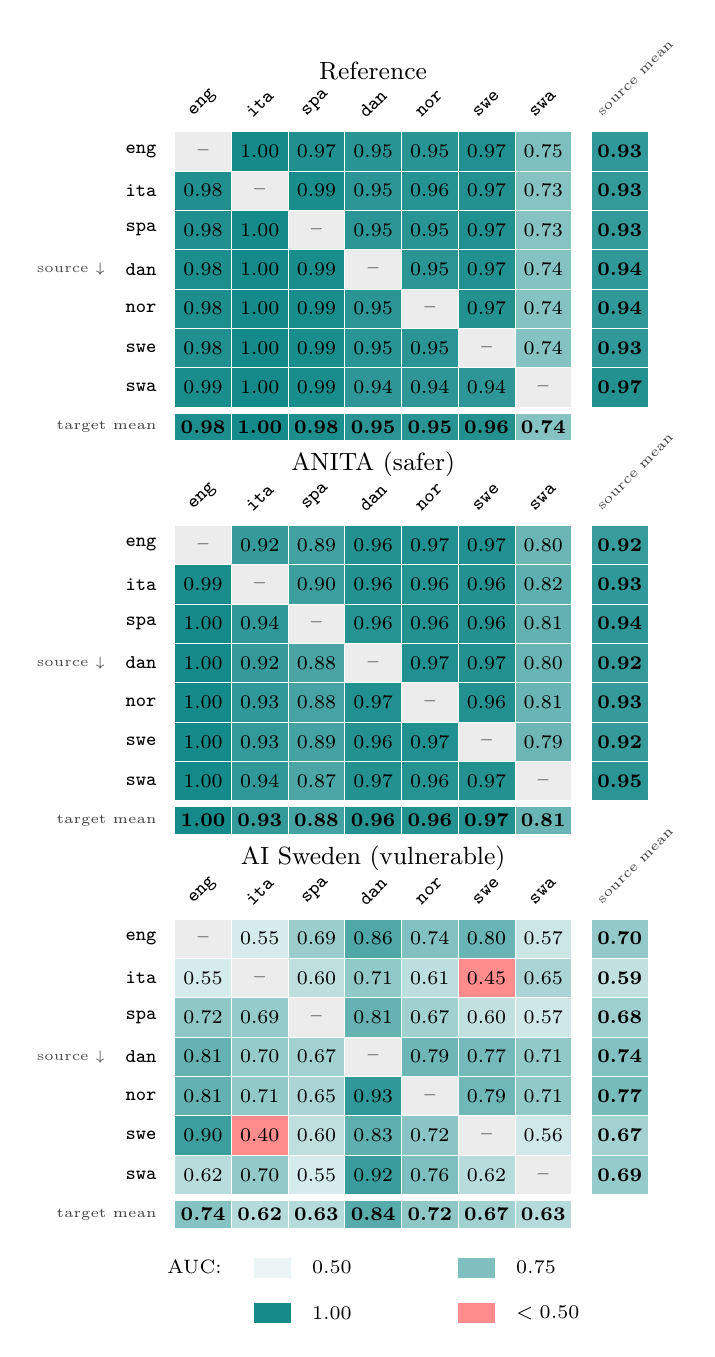
\begin{tikzpicture}[x=0.72cm,y=0.50cm]
\node[font=\small,align=center,text width=7.0cm] at (3.5,1.55) {Reference};
\node[font=\tiny,text=black!70,anchor=east] at (-1.05,-3.5) {source $\downarrow$};
\node[rotate=45,anchor=west,font=\scriptsize] at (0.18,0.25) {\texttt{eng}};
\node[rotate=45,anchor=west,font=\scriptsize] at (1.18,0.25) {\texttt{ita}};
\node[rotate=45,anchor=west,font=\scriptsize] at (2.18,0.25) {\texttt{spa}};
\node[rotate=45,anchor=west,font=\scriptsize] at (3.18,0.25) {\texttt{dan}};
\node[rotate=45,anchor=west,font=\scriptsize] at (4.18,0.25) {\texttt{nor}};
\node[rotate=45,anchor=west,font=\scriptsize] at (5.18,0.25) {\texttt{swe}};
\node[rotate=45,anchor=west,font=\scriptsize] at (6.18,0.25) {\texttt{swa}};
\node[rotate=45,anchor=west,font=\tiny,text=black!75] at (7.38,0.25) {source mean};
\node[anchor=east,font=\scriptsize] at (-0.15,-0.5) {\texttt{eng}};
\fill[gray!15] (0,0) rectangle ++(1,-1);
\draw[white,line width=0.25pt] (0,0) rectangle ++(1,-1);
\node[font=\scriptsize] at (0.5,-0.5) {--};
\fill[teal!92!white] (1,0) rectangle ++(1,-1);
\draw[white,line width=0.25pt] (1,0) rectangle ++(1,-1);
\node[font=\scriptsize] at (1.5,-0.5) {1.00};
\fill[teal!88!white] (2,0) rectangle ++(1,-1);
\draw[white,line width=0.25pt] (2,0) rectangle ++(1,-1);
\node[font=\scriptsize] at (2.5,-0.5) {0.97};
\fill[teal!84!white] (3,0) rectangle ++(1,-1);
\draw[white,line width=0.25pt] (3,0) rectangle ++(1,-1);
\node[font=\scriptsize] at (3.5,-0.5) {0.95};
\fill[teal!84!white] (4,0) rectangle ++(1,-1);
\draw[white,line width=0.25pt] (4,0) rectangle ++(1,-1);
\node[font=\scriptsize] at (4.5,-0.5) {0.95};
\fill[teal!87!white] (5,0) rectangle ++(1,-1);
\draw[white,line width=0.25pt] (5,0) rectangle ++(1,-1);
\node[font=\scriptsize] at (5.5,-0.5) {0.97};
\fill[teal!51!white] (6,0) rectangle ++(1,-1);
\draw[white,line width=0.25pt] (6,0) rectangle ++(1,-1);
\node[font=\scriptsize] at (6.5,-0.5) {0.75};
\fill[teal!81!white] (7.35,0) rectangle ++(1,-1);
\draw[white,line width=0.25pt] (7.35,0) rectangle ++(1,-1);
\node[font=\scriptsize\bfseries] at (7.85,-0.5) {0.93};
\node[anchor=east,font=\scriptsize] at (-0.15,-1.5) {\texttt{ita}};
\fill[teal!88!white] (0,-1) rectangle ++(1,-1);
\draw[white,line width=0.25pt] (0,-1) rectangle ++(1,-1);
\node[font=\scriptsize] at (0.5,-1.5) {0.98};
\fill[gray!15] (1,-1) rectangle ++(1,-1);
\draw[white,line width=0.25pt] (1,-1) rectangle ++(1,-1);
\node[font=\scriptsize] at (1.5,-1.5) {--};
\fill[teal!90!white] (2,-1) rectangle ++(1,-1);
\draw[white,line width=0.25pt] (2,-1) rectangle ++(1,-1);
\node[font=\scriptsize] at (2.5,-1.5) {0.99};
\fill[teal!83!white] (3,-1) rectangle ++(1,-1);
\draw[white,line width=0.25pt] (3,-1) rectangle ++(1,-1);
\node[font=\scriptsize] at (3.5,-1.5) {0.95};
\fill[teal!85!white] (4,-1) rectangle ++(1,-1);
\draw[white,line width=0.25pt] (4,-1) rectangle ++(1,-1);
\node[font=\scriptsize] at (4.5,-1.5) {0.96};
\fill[teal!86!white] (5,-1) rectangle ++(1,-1);
\draw[white,line width=0.25pt] (5,-1) rectangle ++(1,-1);
\node[font=\scriptsize] at (5.5,-1.5) {0.97};
\fill[teal!47!white] (6,-1) rectangle ++(1,-1);
\draw[white,line width=0.25pt] (6,-1) rectangle ++(1,-1);
\node[font=\scriptsize] at (6.5,-1.5) {0.73};
\fill[teal!80!white] (7.35,-1) rectangle ++(1,-1);
\draw[white,line width=0.25pt] (7.35,-1) rectangle ++(1,-1);
\node[font=\scriptsize\bfseries] at (7.85,-1.5) {0.93};
\node[anchor=east,font=\scriptsize] at (-0.15,-2.5) {\texttt{spa}};
\fill[teal!88!white] (0,-2) rectangle ++(1,-1);
\draw[white,line width=0.25pt] (0,-2) rectangle ++(1,-1);
\node[font=\scriptsize] at (0.5,-2.5) {0.98};
\fill[teal!92!white] (1,-2) rectangle ++(1,-1);
\draw[white,line width=0.25pt] (1,-2) rectangle ++(1,-1);
\node[font=\scriptsize] at (1.5,-2.5) {1.00};
\fill[gray!15] (2,-2) rectangle ++(1,-1);
\draw[white,line width=0.25pt] (2,-2) rectangle ++(1,-1);
\node[font=\scriptsize] at (2.5,-2.5) {--};
\fill[teal!83!white] (3,-2) rectangle ++(1,-1);
\draw[white,line width=0.25pt] (3,-2) rectangle ++(1,-1);
\node[font=\scriptsize] at (3.5,-2.5) {0.95};
\fill[teal!84!white] (4,-2) rectangle ++(1,-1);
\draw[white,line width=0.25pt] (4,-2) rectangle ++(1,-1);
\node[font=\scriptsize] at (4.5,-2.5) {0.95};
\fill[teal!87!white] (5,-2) rectangle ++(1,-1);
\draw[white,line width=0.25pt] (5,-2) rectangle ++(1,-1);
\node[font=\scriptsize] at (5.5,-2.5) {0.97};
\fill[teal!47!white] (6,-2) rectangle ++(1,-1);
\draw[white,line width=0.25pt] (6,-2) rectangle ++(1,-1);
\node[font=\scriptsize] at (6.5,-2.5) {0.73};
\fill[teal!80!white] (7.35,-2) rectangle ++(1,-1);
\draw[white,line width=0.25pt] (7.35,-2) rectangle ++(1,-1);
\node[font=\scriptsize\bfseries] at (7.85,-2.5) {0.93};
\node[anchor=east,font=\scriptsize] at (-0.15,-3.5) {\texttt{dan}};
\fill[teal!89!white] (0,-3) rectangle ++(1,-1);
\draw[white,line width=0.25pt] (0,-3) rectangle ++(1,-1);
\node[font=\scriptsize] at (0.5,-3.5) {0.98};
\fill[teal!92!white] (1,-3) rectangle ++(1,-1);
\draw[white,line width=0.25pt] (1,-3) rectangle ++(1,-1);
\node[font=\scriptsize] at (1.5,-3.5) {1.00};
\fill[teal!90!white] (2,-3) rectangle ++(1,-1);
\draw[white,line width=0.25pt] (2,-3) rectangle ++(1,-1);
\node[font=\scriptsize] at (2.5,-3.5) {0.99};
\fill[gray!15] (3,-3) rectangle ++(1,-1);
\draw[white,line width=0.25pt] (3,-3) rectangle ++(1,-1);
\node[font=\scriptsize] at (3.5,-3.5) {--};
\fill[teal!83!white] (4,-3) rectangle ++(1,-1);
\draw[white,line width=0.25pt] (4,-3) rectangle ++(1,-1);
\node[font=\scriptsize] at (4.5,-3.5) {0.95};
\fill[teal!87!white] (5,-3) rectangle ++(1,-1);
\draw[white,line width=0.25pt] (5,-3) rectangle ++(1,-1);
\node[font=\scriptsize] at (5.5,-3.5) {0.97};
\fill[teal!48!white] (6,-3) rectangle ++(1,-1);
\draw[white,line width=0.25pt] (6,-3) rectangle ++(1,-1);
\node[font=\scriptsize] at (6.5,-3.5) {0.74};
\fill[teal!81!white] (7.35,-3) rectangle ++(1,-1);
\draw[white,line width=0.25pt] (7.35,-3) rectangle ++(1,-1);
\node[font=\scriptsize\bfseries] at (7.85,-3.5) {0.94};
\node[anchor=east,font=\scriptsize] at (-0.15,-4.5) {\texttt{nor}};
\fill[teal!89!white] (0,-4) rectangle ++(1,-1);
\draw[white,line width=0.25pt] (0,-4) rectangle ++(1,-1);
\node[font=\scriptsize] at (0.5,-4.5) {0.98};
\fill[teal!92!white] (1,-4) rectangle ++(1,-1);
\draw[white,line width=0.25pt] (1,-4) rectangle ++(1,-1);
\node[font=\scriptsize] at (1.5,-4.5) {1.00};
\fill[teal!90!white] (2,-4) rectangle ++(1,-1);
\draw[white,line width=0.25pt] (2,-4) rectangle ++(1,-1);
\node[font=\scriptsize] at (2.5,-4.5) {0.99};
\fill[teal!83!white] (3,-4) rectangle ++(1,-1);
\draw[white,line width=0.25pt] (3,-4) rectangle ++(1,-1);
\node[font=\scriptsize] at (3.5,-4.5) {0.95};
\fill[gray!15] (4,-4) rectangle ++(1,-1);
\draw[white,line width=0.25pt] (4,-4) rectangle ++(1,-1);
\node[font=\scriptsize] at (4.5,-4.5) {--};
\fill[teal!86!white] (5,-4) rectangle ++(1,-1);
\draw[white,line width=0.25pt] (5,-4) rectangle ++(1,-1);
\node[font=\scriptsize] at (5.5,-4.5) {0.97};
\fill[teal!48!white] (6,-4) rectangle ++(1,-1);
\draw[white,line width=0.25pt] (6,-4) rectangle ++(1,-1);
\node[font=\scriptsize] at (6.5,-4.5) {0.74};
\fill[teal!81!white] (7.35,-4) rectangle ++(1,-1);
\draw[white,line width=0.25pt] (7.35,-4) rectangle ++(1,-1);
\node[font=\scriptsize\bfseries] at (7.85,-4.5) {0.94};
\node[anchor=east,font=\scriptsize] at (-0.15,-5.5) {\texttt{swe}};
\fill[teal!88!white] (0,-5) rectangle ++(1,-1);
\draw[white,line width=0.25pt] (0,-5) rectangle ++(1,-1);
\node[font=\scriptsize] at (0.5,-5.5) {0.98};
\fill[teal!92!white] (1,-5) rectangle ++(1,-1);
\draw[white,line width=0.25pt] (1,-5) rectangle ++(1,-1);
\node[font=\scriptsize] at (1.5,-5.5) {1.00};
\fill[teal!90!white] (2,-5) rectangle ++(1,-1);
\draw[white,line width=0.25pt] (2,-5) rectangle ++(1,-1);
\node[font=\scriptsize] at (2.5,-5.5) {0.99};
\fill[teal!84!white] (3,-5) rectangle ++(1,-1);
\draw[white,line width=0.25pt] (3,-5) rectangle ++(1,-1);
\node[font=\scriptsize] at (3.5,-5.5) {0.95};
\fill[teal!83!white] (4,-5) rectangle ++(1,-1);
\draw[white,line width=0.25pt] (4,-5) rectangle ++(1,-1);
\node[font=\scriptsize] at (4.5,-5.5) {0.95};
\fill[gray!15] (5,-5) rectangle ++(1,-1);
\draw[white,line width=0.25pt] (5,-5) rectangle ++(1,-1);
\node[font=\scriptsize] at (5.5,-5.5) {--};
\fill[teal!48!white] (6,-5) rectangle ++(1,-1);
\draw[white,line width=0.25pt] (6,-5) rectangle ++(1,-1);
\node[font=\scriptsize] at (6.5,-5.5) {0.74};
\fill[teal!81!white] (7.35,-5) rectangle ++(1,-1);
\draw[white,line width=0.25pt] (7.35,-5) rectangle ++(1,-1);
\node[font=\scriptsize\bfseries] at (7.85,-5.5) {0.93};
\node[anchor=east,font=\scriptsize] at (-0.15,-6.5) {\texttt{swa}};
\fill[teal!90!white] (0,-6) rectangle ++(1,-1);
\draw[white,line width=0.25pt] (0,-6) rectangle ++(1,-1);
\node[font=\scriptsize] at (0.5,-6.5) {0.99};
\fill[teal!92!white] (1,-6) rectangle ++(1,-1);
\draw[white,line width=0.25pt] (1,-6) rectangle ++(1,-1);
\node[font=\scriptsize] at (1.5,-6.5) {1.00};
\fill[teal!90!white] (2,-6) rectangle ++(1,-1);
\draw[white,line width=0.25pt] (2,-6) rectangle ++(1,-1);
\node[font=\scriptsize] at (2.5,-6.5) {0.99};
\fill[teal!82!white] (3,-6) rectangle ++(1,-1);
\draw[white,line width=0.25pt] (3,-6) rectangle ++(1,-1);
\node[font=\scriptsize] at (3.5,-6.5) {0.94};
\fill[teal!82!white] (4,-6) rectangle ++(1,-1);
\draw[white,line width=0.25pt] (4,-6) rectangle ++(1,-1);
\node[font=\scriptsize] at (4.5,-6.5) {0.94};
\fill[teal!82!white] (5,-6) rectangle ++(1,-1);
\draw[white,line width=0.25pt] (5,-6) rectangle ++(1,-1);
\node[font=\scriptsize] at (5.5,-6.5) {0.94};
\fill[gray!15] (6,-6) rectangle ++(1,-1);
\draw[white,line width=0.25pt] (6,-6) rectangle ++(1,-1);
\node[font=\scriptsize] at (6.5,-6.5) {--};
\fill[teal!86!white] (7.35,-6) rectangle ++(1,-1);
\draw[white,line width=0.25pt] (7.35,-6) rectangle ++(1,-1);
\node[font=\scriptsize\bfseries] at (7.85,-6.5) {0.97};
\node[anchor=east,font=\tiny,text=black!75] at (-0.15,-7.5) {target mean};
\fill[teal!89!white] (0,-7.15) rectangle ++(1,-0.70);
\draw[white,line width=0.25pt] (0,-7.15) rectangle ++(1,-0.70);
\node[font=\scriptsize\bfseries] at (0.5,-7.5) {0.98};
\fill[teal!92!white] (1,-7.15) rectangle ++(1,-0.70);
\draw[white,line width=0.25pt] (1,-7.15) rectangle ++(1,-0.70);
\node[font=\scriptsize\bfseries] at (1.5,-7.5) {1.00};
\fill[teal!89!white] (2,-7.15) rectangle ++(1,-0.70);
\draw[white,line width=0.25pt] (2,-7.15) rectangle ++(1,-0.70);
\node[font=\scriptsize\bfseries] at (2.5,-7.5) {0.98};
\fill[teal!83!white] (3,-7.15) rectangle ++(1,-0.70);
\draw[white,line width=0.25pt] (3,-7.15) rectangle ++(1,-0.70);
\node[font=\scriptsize\bfseries] at (3.5,-7.5) {0.95};
\fill[teal!84!white] (4,-7.15) rectangle ++(1,-0.70);
\draw[white,line width=0.25pt] (4,-7.15) rectangle ++(1,-0.70);
\node[font=\scriptsize\bfseries] at (4.5,-7.5) {0.95};
\fill[teal!86!white] (5,-7.15) rectangle ++(1,-0.70);
\draw[white,line width=0.25pt] (5,-7.15) rectangle ++(1,-0.70);
\node[font=\scriptsize\bfseries] at (5.5,-7.5) {0.96};
\fill[teal!48!white] (6,-7.15) rectangle ++(1,-0.70);
\draw[white,line width=0.25pt] (6,-7.15) rectangle ++(1,-0.70);
\node[font=\scriptsize\bfseries] at (6.5,-7.5) {0.74};
\node[font=\small,align=center,text width=7.0cm] at (3.5,-8.45) {ANITA (safer)};
\node[font=\tiny,text=black!70,anchor=east] at (-1.05,-13.5) {source $\downarrow$};
\node[rotate=45,anchor=west,font=\scriptsize] at (0.18,-9.75) {\texttt{eng}};
\node[rotate=45,anchor=west,font=\scriptsize] at (1.18,-9.75) {\texttt{ita}};
\node[rotate=45,anchor=west,font=\scriptsize] at (2.18,-9.75) {\texttt{spa}};
\node[rotate=45,anchor=west,font=\scriptsize] at (3.18,-9.75) {\texttt{dan}};
\node[rotate=45,anchor=west,font=\scriptsize] at (4.18,-9.75) {\texttt{nor}};
\node[rotate=45,anchor=west,font=\scriptsize] at (5.18,-9.75) {\texttt{swe}};
\node[rotate=45,anchor=west,font=\scriptsize] at (6.18,-9.75) {\texttt{swa}};
\node[rotate=45,anchor=west,font=\tiny,text=black!75] at (7.38,-9.75) {source mean};
\node[anchor=east,font=\scriptsize] at (-0.15,-10.5) {\texttt{eng}};
\fill[gray!15] (0,-10) rectangle ++(1,-1);
\draw[white,line width=0.25pt] (0,-10) rectangle ++(1,-1);
\node[font=\scriptsize] at (0.5,-10.5) {--};
\fill[teal!79!white] (1,-10) rectangle ++(1,-1);
\draw[white,line width=0.25pt] (1,-10) rectangle ++(1,-1);
\node[font=\scriptsize] at (1.5,-10.5) {0.92};
\fill[teal!74!white] (2,-10) rectangle ++(1,-1);
\draw[white,line width=0.25pt] (2,-10) rectangle ++(1,-1);
\node[font=\scriptsize] at (2.5,-10.5) {0.89};
\fill[teal!86!white] (3,-10) rectangle ++(1,-1);
\draw[white,line width=0.25pt] (3,-10) rectangle ++(1,-1);
\node[font=\scriptsize] at (3.5,-10.5) {0.96};
\fill[teal!87!white] (4,-10) rectangle ++(1,-1);
\draw[white,line width=0.25pt] (4,-10) rectangle ++(1,-1);
\node[font=\scriptsize] at (4.5,-10.5) {0.97};
\fill[teal!87!white] (5,-10) rectangle ++(1,-1);
\draw[white,line width=0.25pt] (5,-10) rectangle ++(1,-1);
\node[font=\scriptsize] at (5.5,-10.5) {0.97};
\fill[teal!58!white] (6,-10) rectangle ++(1,-1);
\draw[white,line width=0.25pt] (6,-10) rectangle ++(1,-1);
\node[font=\scriptsize] at (6.5,-10.5) {0.80};
\fill[teal!78!white] (7.35,-10) rectangle ++(1,-1);
\draw[white,line width=0.25pt] (7.35,-10) rectangle ++(1,-1);
\node[font=\scriptsize\bfseries] at (7.85,-10.5) {0.92};
\node[anchor=east,font=\scriptsize] at (-0.15,-11.5) {\texttt{ita}};
\fill[teal!90!white] (0,-11) rectangle ++(1,-1);
\draw[white,line width=0.25pt] (0,-11) rectangle ++(1,-1);
\node[font=\scriptsize] at (0.5,-11.5) {0.99};
\fill[gray!15] (1,-11) rectangle ++(1,-1);
\draw[white,line width=0.25pt] (1,-11) rectangle ++(1,-1);
\node[font=\scriptsize] at (1.5,-11.5) {--};
\fill[teal!76!white] (2,-11) rectangle ++(1,-1);
\draw[white,line width=0.25pt] (2,-11) rectangle ++(1,-1);
\node[font=\scriptsize] at (2.5,-11.5) {0.90};
\fill[teal!86!white] (3,-11) rectangle ++(1,-1);
\draw[white,line width=0.25pt] (3,-11) rectangle ++(1,-1);
\node[font=\scriptsize] at (3.5,-11.5) {0.96};
\fill[teal!85!white] (4,-11) rectangle ++(1,-1);
\draw[white,line width=0.25pt] (4,-11) rectangle ++(1,-1);
\node[font=\scriptsize] at (4.5,-11.5) {0.96};
\fill[teal!86!white] (5,-11) rectangle ++(1,-1);
\draw[white,line width=0.25pt] (5,-11) rectangle ++(1,-1);
\node[font=\scriptsize] at (5.5,-11.5) {0.96};
\fill[teal!63!white] (6,-11) rectangle ++(1,-1);
\draw[white,line width=0.25pt] (6,-11) rectangle ++(1,-1);
\node[font=\scriptsize] at (6.5,-11.5) {0.82};
\fill[teal!81!white] (7.35,-11) rectangle ++(1,-1);
\draw[white,line width=0.25pt] (7.35,-11) rectangle ++(1,-1);
\node[font=\scriptsize\bfseries] at (7.85,-11.5) {0.93};
\node[anchor=east,font=\scriptsize] at (-0.15,-12.5) {\texttt{spa}};
\fill[teal!92!white] (0,-12) rectangle ++(1,-1);
\draw[white,line width=0.25pt] (0,-12) rectangle ++(1,-1);
\node[font=\scriptsize] at (0.5,-12.5) {1.00};
\fill[teal!81!white] (1,-12) rectangle ++(1,-1);
\draw[white,line width=0.25pt] (1,-12) rectangle ++(1,-1);
\node[font=\scriptsize] at (1.5,-12.5) {0.94};
\fill[gray!15] (2,-12) rectangle ++(1,-1);
\draw[white,line width=0.25pt] (2,-12) rectangle ++(1,-1);
\node[font=\scriptsize] at (2.5,-12.5) {--};
\fill[teal!85!white] (3,-12) rectangle ++(1,-1);
\draw[white,line width=0.25pt] (3,-12) rectangle ++(1,-1);
\node[font=\scriptsize] at (3.5,-12.5) {0.96};
\fill[teal!86!white] (4,-12) rectangle ++(1,-1);
\draw[white,line width=0.25pt] (4,-12) rectangle ++(1,-1);
\node[font=\scriptsize] at (4.5,-12.5) {0.96};
\fill[teal!86!white] (5,-12) rectangle ++(1,-1);
\draw[white,line width=0.25pt] (5,-12) rectangle ++(1,-1);
\node[font=\scriptsize] at (5.5,-12.5) {0.96};
\fill[teal!61!white] (6,-12) rectangle ++(1,-1);
\draw[white,line width=0.25pt] (6,-12) rectangle ++(1,-1);
\node[font=\scriptsize] at (6.5,-12.5) {0.81};
\fill[teal!82!white] (7.35,-12) rectangle ++(1,-1);
\draw[white,line width=0.25pt] (7.35,-12) rectangle ++(1,-1);
\node[font=\scriptsize\bfseries] at (7.85,-12.5) {0.94};
\node[anchor=east,font=\scriptsize] at (-0.15,-13.5) {\texttt{dan}};
\fill[teal!92!white] (0,-13) rectangle ++(1,-1);
\draw[white,line width=0.25pt] (0,-13) rectangle ++(1,-1);
\node[font=\scriptsize] at (0.5,-13.5) {1.00};
\fill[teal!79!white] (1,-13) rectangle ++(1,-1);
\draw[white,line width=0.25pt] (1,-13) rectangle ++(1,-1);
\node[font=\scriptsize] at (1.5,-13.5) {0.92};
\fill[teal!71!white] (2,-13) rectangle ++(1,-1);
\draw[white,line width=0.25pt] (2,-13) rectangle ++(1,-1);
\node[font=\scriptsize] at (2.5,-13.5) {0.88};
\fill[gray!15] (3,-13) rectangle ++(1,-1);
\draw[white,line width=0.25pt] (3,-13) rectangle ++(1,-1);
\node[font=\scriptsize] at (3.5,-13.5) {--};
\fill[teal!87!white] (4,-13) rectangle ++(1,-1);
\draw[white,line width=0.25pt] (4,-13) rectangle ++(1,-1);
\node[font=\scriptsize] at (4.5,-13.5) {0.97};
\fill[teal!86!white] (5,-13) rectangle ++(1,-1);
\draw[white,line width=0.25pt] (5,-13) rectangle ++(1,-1);
\node[font=\scriptsize] at (5.5,-13.5) {0.97};
\fill[teal!59!white] (6,-13) rectangle ++(1,-1);
\draw[white,line width=0.25pt] (6,-13) rectangle ++(1,-1);
\node[font=\scriptsize] at (6.5,-13.5) {0.80};
\fill[teal!79!white] (7.35,-13) rectangle ++(1,-1);
\draw[white,line width=0.25pt] (7.35,-13) rectangle ++(1,-1);
\node[font=\scriptsize\bfseries] at (7.85,-13.5) {0.92};
\node[anchor=east,font=\scriptsize] at (-0.15,-14.5) {\texttt{nor}};
\fill[teal!92!white] (0,-14) rectangle ++(1,-1);
\draw[white,line width=0.25pt] (0,-14) rectangle ++(1,-1);
\node[font=\scriptsize] at (0.5,-14.5) {1.00};
\fill[teal!81!white] (1,-14) rectangle ++(1,-1);
\draw[white,line width=0.25pt] (1,-14) rectangle ++(1,-1);
\node[font=\scriptsize] at (1.5,-14.5) {0.93};
\fill[teal!72!white] (2,-14) rectangle ++(1,-1);
\draw[white,line width=0.25pt] (2,-14) rectangle ++(1,-1);
\node[font=\scriptsize] at (2.5,-14.5) {0.88};
\fill[teal!87!white] (3,-14) rectangle ++(1,-1);
\draw[white,line width=0.25pt] (3,-14) rectangle ++(1,-1);
\node[font=\scriptsize] at (3.5,-14.5) {0.97};
\fill[gray!15] (4,-14) rectangle ++(1,-1);
\draw[white,line width=0.25pt] (4,-14) rectangle ++(1,-1);
\node[font=\scriptsize] at (4.5,-14.5) {--};
\fill[teal!86!white] (5,-14) rectangle ++(1,-1);
\draw[white,line width=0.25pt] (5,-14) rectangle ++(1,-1);
\node[font=\scriptsize] at (5.5,-14.5) {0.96};
\fill[teal!59!white] (6,-14) rectangle ++(1,-1);
\draw[white,line width=0.25pt] (6,-14) rectangle ++(1,-1);
\node[font=\scriptsize] at (6.5,-14.5) {0.81};
\fill[teal!79!white] (7.35,-14) rectangle ++(1,-1);
\draw[white,line width=0.25pt] (7.35,-14) rectangle ++(1,-1);
\node[font=\scriptsize\bfseries] at (7.85,-14.5) {0.93};
\node[anchor=east,font=\scriptsize] at (-0.15,-15.5) {\texttt{swe}};
\fill[teal!92!white] (0,-15) rectangle ++(1,-1);
\draw[white,line width=0.25pt] (0,-15) rectangle ++(1,-1);
\node[font=\scriptsize] at (0.5,-15.5) {1.00};
\fill[teal!80!white] (1,-15) rectangle ++(1,-1);
\draw[white,line width=0.25pt] (1,-15) rectangle ++(1,-1);
\node[font=\scriptsize] at (1.5,-15.5) {0.93};
\fill[teal!73!white] (2,-15) rectangle ++(1,-1);
\draw[white,line width=0.25pt] (2,-15) rectangle ++(1,-1);
\node[font=\scriptsize] at (2.5,-15.5) {0.89};
\fill[teal!86!white] (3,-15) rectangle ++(1,-1);
\draw[white,line width=0.25pt] (3,-15) rectangle ++(1,-1);
\node[font=\scriptsize] at (3.5,-15.5) {0.96};
\fill[teal!87!white] (4,-15) rectangle ++(1,-1);
\draw[white,line width=0.25pt] (4,-15) rectangle ++(1,-1);
\node[font=\scriptsize] at (4.5,-15.5) {0.97};
\fill[gray!15] (5,-15) rectangle ++(1,-1);
\draw[white,line width=0.25pt] (5,-15) rectangle ++(1,-1);
\node[font=\scriptsize] at (5.5,-15.5) {--};
\fill[teal!57!white] (6,-15) rectangle ++(1,-1);
\draw[white,line width=0.25pt] (6,-15) rectangle ++(1,-1);
\node[font=\scriptsize] at (6.5,-15.5) {0.79};
\fill[teal!79!white] (7.35,-15) rectangle ++(1,-1);
\draw[white,line width=0.25pt] (7.35,-15) rectangle ++(1,-1);
\node[font=\scriptsize\bfseries] at (7.85,-15.5) {0.92};
\node[anchor=east,font=\scriptsize] at (-0.15,-16.5) {\texttt{swa}};
\fill[teal!92!white] (0,-16) rectangle ++(1,-1);
\draw[white,line width=0.25pt] (0,-16) rectangle ++(1,-1);
\node[font=\scriptsize] at (0.5,-16.5) {1.00};
\fill[teal!81!white] (1,-16) rectangle ++(1,-1);
\draw[white,line width=0.25pt] (1,-16) rectangle ++(1,-1);
\node[font=\scriptsize] at (1.5,-16.5) {0.94};
\fill[teal!70!white] (2,-16) rectangle ++(1,-1);
\draw[white,line width=0.25pt] (2,-16) rectangle ++(1,-1);
\node[font=\scriptsize] at (2.5,-16.5) {0.87};
\fill[teal!86!white] (3,-16) rectangle ++(1,-1);
\draw[white,line width=0.25pt] (3,-16) rectangle ++(1,-1);
\node[font=\scriptsize] at (3.5,-16.5) {0.97};
\fill[teal!85!white] (4,-16) rectangle ++(1,-1);
\draw[white,line width=0.25pt] (4,-16) rectangle ++(1,-1);
\node[font=\scriptsize] at (4.5,-16.5) {0.96};
\fill[teal!86!white] (5,-16) rectangle ++(1,-1);
\draw[white,line width=0.25pt] (5,-16) rectangle ++(1,-1);
\node[font=\scriptsize] at (5.5,-16.5) {0.97};
\fill[gray!15] (6,-16) rectangle ++(1,-1);
\draw[white,line width=0.25pt] (6,-16) rectangle ++(1,-1);
\node[font=\scriptsize] at (6.5,-16.5) {--};
\fill[teal!83!white] (7.35,-16) rectangle ++(1,-1);
\draw[white,line width=0.25pt] (7.35,-16) rectangle ++(1,-1);
\node[font=\scriptsize\bfseries] at (7.85,-16.5) {0.95};
\node[anchor=east,font=\tiny,text=black!75] at (-0.15,-17.5) {target mean};
\fill[teal!92!white] (0,-17.15) rectangle ++(1,-0.70);
\draw[white,line width=0.25pt] (0,-17.15) rectangle ++(1,-0.70);
\node[font=\scriptsize\bfseries] at (0.5,-17.5) {1.00};
\fill[teal!80!white] (1,-17.15) rectangle ++(1,-0.70);
\draw[white,line width=0.25pt] (1,-17.15) rectangle ++(1,-0.70);
\node[font=\scriptsize\bfseries] at (1.5,-17.5) {0.93};
\fill[teal!73!white] (2,-17.15) rectangle ++(1,-0.70);
\draw[white,line width=0.25pt] (2,-17.15) rectangle ++(1,-0.70);
\node[font=\scriptsize\bfseries] at (2.5,-17.5) {0.88};
\fill[teal!86!white] (3,-17.15) rectangle ++(1,-0.70);
\draw[white,line width=0.25pt] (3,-17.15) rectangle ++(1,-0.70);
\node[font=\scriptsize\bfseries] at (3.5,-17.5) {0.96};
\fill[teal!86!white] (4,-17.15) rectangle ++(1,-0.70);
\draw[white,line width=0.25pt] (4,-17.15) rectangle ++(1,-0.70);
\node[font=\scriptsize\bfseries] at (4.5,-17.5) {0.96};
\fill[teal!86!white] (5,-17.15) rectangle ++(1,-0.70);
\draw[white,line width=0.25pt] (5,-17.15) rectangle ++(1,-0.70);
\node[font=\scriptsize\bfseries] at (5.5,-17.5) {0.97};
\fill[teal!59!white] (6,-17.15) rectangle ++(1,-0.70);
\draw[white,line width=0.25pt] (6,-17.15) rectangle ++(1,-0.70);
\node[font=\scriptsize\bfseries] at (6.5,-17.5) {0.81};
\node[font=\small,align=center,text width=7.0cm] at (3.5,-18.45) {AI Sweden (vulnerable)};
\node[font=\tiny,text=black!70,anchor=east] at (-1.05,-23.5) {source $\downarrow$};
\node[rotate=45,anchor=west,font=\scriptsize] at (0.18,-19.75) {\texttt{eng}};
\node[rotate=45,anchor=west,font=\scriptsize] at (1.18,-19.75) {\texttt{ita}};
\node[rotate=45,anchor=west,font=\scriptsize] at (2.18,-19.75) {\texttt{spa}};
\node[rotate=45,anchor=west,font=\scriptsize] at (3.18,-19.75) {\texttt{dan}};
\node[rotate=45,anchor=west,font=\scriptsize] at (4.18,-19.75) {\texttt{nor}};
\node[rotate=45,anchor=west,font=\scriptsize] at (5.18,-19.75) {\texttt{swe}};
\node[rotate=45,anchor=west,font=\scriptsize] at (6.18,-19.75) {\texttt{swa}};
\node[rotate=45,anchor=west,font=\tiny,text=black!75] at (7.38,-19.75) {source mean};
\node[anchor=east,font=\scriptsize] at (-0.15,-20.5) {\texttt{eng}};
\fill[gray!15] (0,-20) rectangle ++(1,-1);
\draw[white,line width=0.25pt] (0,-20) rectangle ++(1,-1);
\node[font=\scriptsize] at (0.5,-20.5) {--};
\fill[teal!16!white] (1,-20) rectangle ++(1,-1);
\draw[white,line width=0.25pt] (1,-20) rectangle ++(1,-1);
\node[font=\scriptsize] at (1.5,-20.5) {0.55};
\fill[teal!39!white] (2,-20) rectangle ++(1,-1);
\draw[white,line width=0.25pt] (2,-20) rectangle ++(1,-1);
\node[font=\scriptsize] at (2.5,-20.5) {0.69};
\fill[teal!69!white] (3,-20) rectangle ++(1,-1);
\draw[white,line width=0.25pt] (3,-20) rectangle ++(1,-1);
\node[font=\scriptsize] at (3.5,-20.5) {0.86};
\fill[teal!49!white] (4,-20) rectangle ++(1,-1);
\draw[white,line width=0.25pt] (4,-20) rectangle ++(1,-1);
\node[font=\scriptsize] at (4.5,-20.5) {0.74};
\fill[teal!59!white] (5,-20) rectangle ++(1,-1);
\draw[white,line width=0.25pt] (5,-20) rectangle ++(1,-1);
\node[font=\scriptsize] at (5.5,-20.5) {0.80};
\fill[teal!20!white] (6,-20) rectangle ++(1,-1);
\draw[white,line width=0.25pt] (6,-20) rectangle ++(1,-1);
\node[font=\scriptsize] at (6.5,-20.5) {0.57};
\fill[teal!42!white] (7.35,-20) rectangle ++(1,-1);
\draw[white,line width=0.25pt] (7.35,-20) rectangle ++(1,-1);
\node[font=\scriptsize\bfseries] at (7.85,-20.5) {0.70};
\node[anchor=east,font=\scriptsize] at (-0.15,-21.5) {\texttt{ita}};
\fill[teal!16!white] (0,-21) rectangle ++(1,-1);
\draw[white,line width=0.25pt] (0,-21) rectangle ++(1,-1);
\node[font=\scriptsize] at (0.5,-21.5) {0.55};
\fill[gray!15] (1,-21) rectangle ++(1,-1);
\draw[white,line width=0.25pt] (1,-21) rectangle ++(1,-1);
\node[font=\scriptsize] at (1.5,-21.5) {--};
\fill[teal!25!white] (2,-21) rectangle ++(1,-1);
\draw[white,line width=0.25pt] (2,-21) rectangle ++(1,-1);
\node[font=\scriptsize] at (2.5,-21.5) {0.60};
\fill[teal!43!white] (3,-21) rectangle ++(1,-1);
\draw[white,line width=0.25pt] (3,-21) rectangle ++(1,-1);
\node[font=\scriptsize] at (3.5,-21.5) {0.71};
\fill[teal!26!white] (4,-21) rectangle ++(1,-1);
\draw[white,line width=0.25pt] (4,-21) rectangle ++(1,-1);
\node[font=\scriptsize] at (4.5,-21.5) {0.61};
\fill[red!45!white] (5,-21) rectangle ++(1,-1);
\draw[white,line width=0.25pt] (5,-21) rectangle ++(1,-1);
\node[font=\scriptsize] at (5.5,-21.5) {0.45};
\fill[teal!33!white] (6,-21) rectangle ++(1,-1);
\draw[white,line width=0.25pt] (6,-21) rectangle ++(1,-1);
\node[font=\scriptsize] at (6.5,-21.5) {0.65};
\fill[teal!24!white] (7.35,-21) rectangle ++(1,-1);
\draw[white,line width=0.25pt] (7.35,-21) rectangle ++(1,-1);
\node[font=\scriptsize\bfseries] at (7.85,-21.5) {0.59};
\node[anchor=east,font=\scriptsize] at (-0.15,-22.5) {\texttt{spa}};
\fill[teal!44!white] (0,-22) rectangle ++(1,-1);
\draw[white,line width=0.25pt] (0,-22) rectangle ++(1,-1);
\node[font=\scriptsize] at (0.5,-22.5) {0.72};
\fill[teal!41!white] (1,-22) rectangle ++(1,-1);
\draw[white,line width=0.25pt] (1,-22) rectangle ++(1,-1);
\node[font=\scriptsize] at (1.5,-22.5) {0.69};
\fill[gray!15] (2,-22) rectangle ++(1,-1);
\draw[white,line width=0.25pt] (2,-22) rectangle ++(1,-1);
\node[font=\scriptsize] at (2.5,-22.5) {--};
\fill[teal!60!white] (3,-22) rectangle ++(1,-1);
\draw[white,line width=0.25pt] (3,-22) rectangle ++(1,-1);
\node[font=\scriptsize] at (3.5,-22.5) {0.81};
\fill[teal!37!white] (4,-22) rectangle ++(1,-1);
\draw[white,line width=0.25pt] (4,-22) rectangle ++(1,-1);
\node[font=\scriptsize] at (4.5,-22.5) {0.67};
\fill[teal!24!white] (5,-22) rectangle ++(1,-1);
\draw[white,line width=0.25pt] (5,-22) rectangle ++(1,-1);
\node[font=\scriptsize] at (5.5,-22.5) {0.60};
\fill[teal!19!white] (6,-22) rectangle ++(1,-1);
\draw[white,line width=0.25pt] (6,-22) rectangle ++(1,-1);
\node[font=\scriptsize] at (6.5,-22.5) {0.57};
\fill[teal!38!white] (7.35,-22) rectangle ++(1,-1);
\draw[white,line width=0.25pt] (7.35,-22) rectangle ++(1,-1);
\node[font=\scriptsize\bfseries] at (7.85,-22.5) {0.68};
\node[anchor=east,font=\scriptsize] at (-0.15,-23.5) {\texttt{dan}};
\fill[teal!60!white] (0,-23) rectangle ++(1,-1);
\draw[white,line width=0.25pt] (0,-23) rectangle ++(1,-1);
\node[font=\scriptsize] at (0.5,-23.5) {0.81};
\fill[teal!41!white] (1,-23) rectangle ++(1,-1);
\draw[white,line width=0.25pt] (1,-23) rectangle ++(1,-1);
\node[font=\scriptsize] at (1.5,-23.5) {0.70};
\fill[teal!36!white] (2,-23) rectangle ++(1,-1);
\draw[white,line width=0.25pt] (2,-23) rectangle ++(1,-1);
\node[font=\scriptsize] at (2.5,-23.5) {0.67};
\fill[gray!15] (3,-23) rectangle ++(1,-1);
\draw[white,line width=0.25pt] (3,-23) rectangle ++(1,-1);
\node[font=\scriptsize] at (3.5,-23.5) {--};
\fill[teal!57!white] (4,-23) rectangle ++(1,-1);
\draw[white,line width=0.25pt] (4,-23) rectangle ++(1,-1);
\node[font=\scriptsize] at (4.5,-23.5) {0.79};
\fill[teal!54!white] (5,-23) rectangle ++(1,-1);
\draw[white,line width=0.25pt] (5,-23) rectangle ++(1,-1);
\node[font=\scriptsize] at (5.5,-23.5) {0.77};
\fill[teal!43!white] (6,-23) rectangle ++(1,-1);
\draw[white,line width=0.25pt] (6,-23) rectangle ++(1,-1);
\node[font=\scriptsize] at (6.5,-23.5) {0.71};
\fill[teal!49!white] (7.35,-23) rectangle ++(1,-1);
\draw[white,line width=0.25pt] (7.35,-23) rectangle ++(1,-1);
\node[font=\scriptsize\bfseries] at (7.85,-23.5) {0.74};
\node[anchor=east,font=\scriptsize] at (-0.15,-24.5) {\texttt{nor}};
\fill[teal!61!white] (0,-24) rectangle ++(1,-1);
\draw[white,line width=0.25pt] (0,-24) rectangle ++(1,-1);
\node[font=\scriptsize] at (0.5,-24.5) {0.81};
\fill[teal!43!white] (1,-24) rectangle ++(1,-1);
\draw[white,line width=0.25pt] (1,-24) rectangle ++(1,-1);
\node[font=\scriptsize] at (1.5,-24.5) {0.71};
\fill[teal!33!white] (2,-24) rectangle ++(1,-1);
\draw[white,line width=0.25pt] (2,-24) rectangle ++(1,-1);
\node[font=\scriptsize] at (2.5,-24.5) {0.65};
\fill[teal!81!white] (3,-24) rectangle ++(1,-1);
\draw[white,line width=0.25pt] (3,-24) rectangle ++(1,-1);
\node[font=\scriptsize] at (3.5,-24.5) {0.93};
\fill[gray!15] (4,-24) rectangle ++(1,-1);
\draw[white,line width=0.25pt] (4,-24) rectangle ++(1,-1);
\node[font=\scriptsize] at (4.5,-24.5) {--};
\fill[teal!56!white] (5,-24) rectangle ++(1,-1);
\draw[white,line width=0.25pt] (5,-24) rectangle ++(1,-1);
\node[font=\scriptsize] at (5.5,-24.5) {0.79};
\fill[teal!43!white] (6,-24) rectangle ++(1,-1);
\draw[white,line width=0.25pt] (6,-24) rectangle ++(1,-1);
\node[font=\scriptsize] at (6.5,-24.5) {0.71};
\fill[teal!53!white] (7.35,-24) rectangle ++(1,-1);
\draw[white,line width=0.25pt] (7.35,-24) rectangle ++(1,-1);
\node[font=\scriptsize\bfseries] at (7.85,-24.5) {0.77};
\node[anchor=east,font=\scriptsize] at (-0.15,-25.5) {\texttt{swe}};
\fill[teal!76!white] (0,-25) rectangle ++(1,-1);
\draw[white,line width=0.25pt] (0,-25) rectangle ++(1,-1);
\node[font=\scriptsize] at (0.5,-25.5) {0.90};
\fill[red!45!white] (1,-25) rectangle ++(1,-1);
\draw[white,line width=0.25pt] (1,-25) rectangle ++(1,-1);
\node[font=\scriptsize] at (1.5,-25.5) {0.40};
\fill[teal!25!white] (2,-25) rectangle ++(1,-1);
\draw[white,line width=0.25pt] (2,-25) rectangle ++(1,-1);
\node[font=\scriptsize] at (2.5,-25.5) {0.60};
\fill[teal!63!white] (3,-25) rectangle ++(1,-1);
\draw[white,line width=0.25pt] (3,-25) rectangle ++(1,-1);
\node[font=\scriptsize] at (3.5,-25.5) {0.83};
\fill[teal!46!white] (4,-25) rectangle ++(1,-1);
\draw[white,line width=0.25pt] (4,-25) rectangle ++(1,-1);
\node[font=\scriptsize] at (4.5,-25.5) {0.72};
\fill[gray!15] (5,-25) rectangle ++(1,-1);
\draw[white,line width=0.25pt] (5,-25) rectangle ++(1,-1);
\node[font=\scriptsize] at (5.5,-25.5) {--};
\fill[teal!18!white] (6,-25) rectangle ++(1,-1);
\draw[white,line width=0.25pt] (6,-25) rectangle ++(1,-1);
\node[font=\scriptsize] at (6.5,-25.5) {0.56};
\fill[teal!36!white] (7.35,-25) rectangle ++(1,-1);
\draw[white,line width=0.25pt] (7.35,-25) rectangle ++(1,-1);
\node[font=\scriptsize\bfseries] at (7.85,-25.5) {0.67};
\node[anchor=east,font=\scriptsize] at (-0.15,-26.5) {\texttt{swa}};
\fill[teal!28!white] (0,-26) rectangle ++(1,-1);
\draw[white,line width=0.25pt] (0,-26) rectangle ++(1,-1);
\node[font=\scriptsize] at (0.5,-26.5) {0.62};
\fill[teal!42!white] (1,-26) rectangle ++(1,-1);
\draw[white,line width=0.25pt] (1,-26) rectangle ++(1,-1);
\node[font=\scriptsize] at (1.5,-26.5) {0.70};
\fill[teal!16!white] (2,-26) rectangle ++(1,-1);
\draw[white,line width=0.25pt] (2,-26) rectangle ++(1,-1);
\node[font=\scriptsize] at (2.5,-26.5) {0.55};
\fill[teal!78!white] (3,-26) rectangle ++(1,-1);
\draw[white,line width=0.25pt] (3,-26) rectangle ++(1,-1);
\node[font=\scriptsize] at (3.5,-26.5) {0.92};
\fill[teal!51!white] (4,-26) rectangle ++(1,-1);
\draw[white,line width=0.25pt] (4,-26) rectangle ++(1,-1);
\node[font=\scriptsize] at (4.5,-26.5) {0.76};
\fill[teal!28!white] (5,-26) rectangle ++(1,-1);
\draw[white,line width=0.25pt] (5,-26) rectangle ++(1,-1);
\node[font=\scriptsize] at (5.5,-26.5) {0.62};
\fill[gray!15] (6,-26) rectangle ++(1,-1);
\draw[white,line width=0.25pt] (6,-26) rectangle ++(1,-1);
\node[font=\scriptsize] at (6.5,-26.5) {--};
\fill[teal!41!white] (7.35,-26) rectangle ++(1,-1);
\draw[white,line width=0.25pt] (7.35,-26) rectangle ++(1,-1);
\node[font=\scriptsize\bfseries] at (7.85,-26.5) {0.69};
\node[anchor=east,font=\tiny,text=black!75] at (-0.15,-27.5) {target mean};
\fill[teal!48!white] (0,-27.15) rectangle ++(1,-0.70);
\draw[white,line width=0.25pt] (0,-27.15) rectangle ++(1,-0.70);
\node[font=\scriptsize\bfseries] at (0.5,-27.5) {0.74};
\fill[teal!29!white] (1,-27.15) rectangle ++(1,-0.70);
\draw[white,line width=0.25pt] (1,-27.15) rectangle ++(1,-0.70);
\node[font=\scriptsize\bfseries] at (1.5,-27.5) {0.62};
\fill[teal!29!white] (2,-27.15) rectangle ++(1,-0.70);
\draw[white,line width=0.25pt] (2,-27.15) rectangle ++(1,-0.70);
\node[font=\scriptsize\bfseries] at (2.5,-27.5) {0.63};
\fill[teal!66!white] (3,-27.15) rectangle ++(1,-0.70);
\draw[white,line width=0.25pt] (3,-27.15) rectangle ++(1,-0.70);
\node[font=\scriptsize\bfseries] at (3.5,-27.5) {0.84};
\fill[teal!44!white] (4,-27.15) rectangle ++(1,-0.70);
\draw[white,line width=0.25pt] (4,-27.15) rectangle ++(1,-0.70);
\node[font=\scriptsize\bfseries] at (4.5,-27.5) {0.72};
\fill[teal!37!white] (5,-27.15) rectangle ++(1,-0.70);
\draw[white,line width=0.25pt] (5,-27.15) rectangle ++(1,-0.70);
\node[font=\scriptsize\bfseries] at (5.5,-27.5) {0.67};
\fill[teal!29!white] (6,-27.15) rectangle ++(1,-0.70);
\draw[white,line width=0.25pt] (6,-27.15) rectangle ++(1,-0.70);
\node[font=\scriptsize\bfseries] at (6.5,-27.5) {0.63};
\node[font=\scriptsize,anchor=east] at (1.0,-28.85) {AUC:};
\fill[teal!8!white] (1.4,-29.12) rectangle ++(0.65,0.52);
\node[font=\scriptsize,anchor=west] at (2.25,-28.86) {$0.50$};
\fill[teal!50!white] (5.0,-29.12) rectangle ++(0.65,0.52);
\node[font=\scriptsize,anchor=west] at (5.85,-28.86) {$0.75$};
\fill[teal!92!white] (1.4,-30.27) rectangle ++(0.65,0.52);
\node[font=\scriptsize,anchor=west] at (2.25,-30.01) {$1.00$};
\fill[red!45!white] (5.0,-30.27) rectangle ++(0.65,0.52);
\node[font=\scriptsize,anchor=west] at (5.85,-30.01) {$<0.50$};
\end{tikzpicture}
\caption[Cross-lingual transfer matrices for refusal-outcome directions]{Cross-lingual transfer matrices for all 126 ordered language pairs. Each row estimates a direction in the source language; each column evaluates it in a different target language. Cells report AUC and the diagonal is omitted because within-language values are in-sample. Bold right margins average each source row; bold bottom margins average transfer into each target column.}
\label{fig:mechanistic-transfer-matrices}
\fonte{Prepared by the author (2026), using the transfer protocol of \textcite{wangRefusalDirectionUniversal2025}.}
\end{figure}
}

\newcommand{\MechTransferAnalysisText}{%
Figure~\ref{fig:mechanistic-transfer-matrices} expands the mean transfer scores into all 126 ordered source--target language pairs. Reading across a row asks whether a direction estimated in one source language transfers broadly; reading down a column asks whether a target language is separable under directions learned elsewhere. The reference and ANITA have uniformly strong rows, whereas AI Sweden is heterogeneous: its Italian (\texttt{ita}) source direction has the lowest mean transfer AUC ($0.59$), while its Norwegian (\texttt{nor}) source direction has the highest ($0.77$). The source--target distinction also reveals a pattern hidden by a single mean. For the reference, Swahili is a strong \emph{source} direction (mean transfer $0.97$) but a difficult \emph{target} (mean transfer-in $0.74$); ANITA shows the same asymmetry ($0.95$ versus $0.81$). This indicates that a language can yield a portable contrast even when examples in that language remain comparatively difficult to separate with directions estimated elsewhere.
}

\newcommand{\MechSeparabilityAsrFigure}{%
\begin{figure}[htbp]
\centering
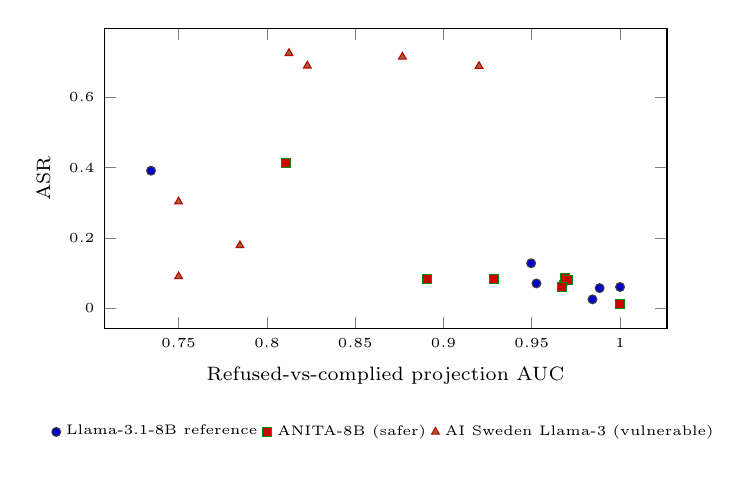
\begin{tikzpicture}
\begin{axis}[width=0.72\linewidth,height=5.4cm,
xlabel={Refused-vs-complied projection AUC},ylabel={ASR},
label style={font=\scriptsize},tick label style={font=\tiny},
legend style={font=\tiny,at={(0.5,-0.28)},anchor=north,draw=none,fill=none,legend columns=3}]
\addplot+[only marks,mark=*,mark size=1.6pt,black!75!white] coordinates {(0.9496527777777778,0.1282051282051282) (0.984375,0.025559105431309903) (1.0,0.06070287539936102) (0.9526515151515151,0.0707395498392283) (0.9884259259259259,0.05750798722044728) (0.734375,0.39158576051779936) (0.9678030303030303,0.07096774193548387)};
\addlegendentry{Llama-3.1-8B reference}
\addplot+[only marks,mark=square*,mark size=1.6pt,green!55!black] coordinates {(0.96875,0.08653846153846154) (1.0,0.012779552715654952) (0.9288194444444444,0.08306709265175719) (0.9704861111111112,0.08038585209003216) (0.890625,0.08306709265175719) (0.8107638888888888,0.41423948220064727) (0.9671052631578947,0.06129032258064516)};
\addlegendentry{ANITA-8B (safer)}
\addplot+[only marks,mark=triangle*,mark size=1.6pt,red!75!black] coordinates {(0.9201388888888888,0.6891025641025641) (0.8767361111111112,0.7156549520766773) (0.7847222222222222,0.17891373801916932) (0.8229166666666666,0.6903225806451613) (0.75,0.3035143769968051) (0.75,0.09061488673139159) (0.8125,0.7258064516129032)};
\addlegendentry{AI Sweden Llama-3 (vulnerable)}
\end{axis}
\end{tikzpicture}
\caption[Refusal-signal separability versus ASR]{In-sample refusal-signal separability versus behavioral ASR across 21 model--language cells. The pooled association is negative, but the within-model direction is heterogeneous; Spearman coefficients are reported in the text.}
\label{fig:mechanistic-separability-vs-asr}
\fonte{Prepared by the author (2026).}
\end{figure}
}

\newcommand{\MechLayerSweepFigure}{%
\begin{figure}[htbp]
\centering
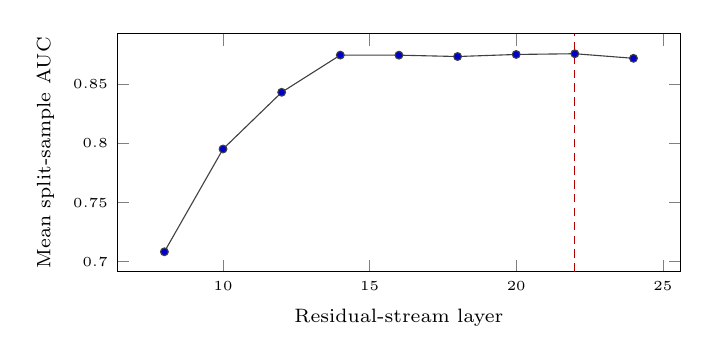
\begin{tikzpicture}
\begin{axis}[width=0.72\linewidth,height=4.6cm,
xlabel={Residual-stream layer},ylabel={Mean split-sample AUC},
label style={font=\scriptsize},tick label style={font=\tiny}]
\addplot+[mark=*,mark size=1.4pt,black!75!white] coordinates {(8,0.7083884479717814) (10,0.7952374790495909) (12,0.8431731790945042) (14,0.8745912616254232) (16,0.8745210846013124) (18,0.8733831898298773) (20,0.8751263186433994) (22,0.8757466150711491) (24,0.871869077743819)};
\draw[densely dashed,red!70!black] (axis cs:22,\pgfkeysvalueof{/pgfplots/ymin}) -- (axis cs:22,\pgfkeysvalueof{/pgfplots/ymax});
\end{axis}
\end{tikzpicture}
\caption[Layer sweep for the refusal-outcome direction]{Layer sweep: mean split-sample refused-versus-complied AUC across the three models. The dashed line marks the layer selected using these same test splits, so the peak is a selection criterion rather than an independent performance estimate.}
\label{fig:mechanistic-layer-sweep-legacy}
\fonte{Prepared by the author (2026).}
\end{figure}
}

\newcommand{\MechRefusalProjectionsTable}{%
\begin{table}[htbp]
\centering
\scriptsize
\caption[Refusal-outcome direction diagnostics per model--language cell]{Refusal-outcome direction diagnostics per model--language cell: in-sample within-language projection AUC, mean cross-lingual transfer AUC into the cell, cosine to the aligned-language direction, and frozen behavioral ASR.}
\label{tab:mechanistic-refusal-projections-legacy}
\begin{tabular}{llrrrr}
\toprule
Model & Lang. & AUC & Transfer-in & Cosine & ASR \\
\midrule
Llama-3.1-8B reference & \texttt{eng} & 0.98 & 0.98 & 1.00 & 2.6\% \\
 & \texttt{ita} & 1.00 & 1.00 & 0.68 & 6.1\% \\
 & \texttt{spa} & 0.99 & 0.98 & 0.69 & 5.8\% \\
 & \texttt{dan} & 0.95 & 0.95 & 0.69 & 12.8\% \\
 & \texttt{nor} & 0.95 & 0.95 & 0.70 & 7.1\% \\
 & \texttt{swe} & 0.97 & 0.96 & 0.74 & 7.1\% \\
 & \texttt{swa} & 0.73 & 0.74 & 0.51 & 39.2\% \\
\midrule
ANITA-8B (safer) & \texttt{eng} & 1.00 & 1.00 & 0.73 & 1.3\% \\
 & \texttt{ita} & 0.93 & 0.93 & 1.00 & 8.3\% \\
 & \texttt{spa} & 0.89 & 0.88 & 0.90 & 8.3\% \\
 & \texttt{dan} & 0.97 & 0.96 & 0.84 & 8.7\% \\
 & \texttt{nor} & 0.97 & 0.96 & 0.84 & 8.0\% \\
 & \texttt{swe} & 0.97 & 0.97 & 0.85 & 6.1\% \\
 & \texttt{swa} & 0.81 & 0.81 & 0.69 & 41.4\% \\
\midrule
AI Sweden Llama-3 (vulnerable) & \texttt{eng} & 0.88 & 0.74 & 0.69 & 71.6\% \\
 & \texttt{ita} & 0.78 & 0.62 & -0.10 & 17.9\% \\
 & \texttt{spa} & 0.75 & 0.63 & 0.11 & 30.4\% \\
 & \texttt{dan} & 0.92 & 0.84 & 0.53 & 68.9\% \\
 & \texttt{nor} & 0.82 & 0.72 & 0.44 & 69.0\% \\
 & \texttt{swe} & 0.81 & 0.67 & 1.00 & 72.6\% \\
 & \texttt{swa} & 0.75 & 0.63 & 0.08 & 9.1\% \\
\bottomrule
\end{tabular}
\fonte{Prepared by the author (2026).}
\end{table}
}

\newcommand{\MechLanguageDirectionSimilarityTable}{%
\begin{table}[htbp]
\centering
\scriptsize
\caption[Cross-lingual refusal-direction cosine similarity]{Cosine similarity of each attack language's refusal-outcome direction to the model's aligned-language direction and to the model's pooled direction.}
\label{tab:mechanistic-language-direction-similarity}
\begin{tabular}{llrr}
\toprule
Model & Lang. & Cos.\ aligned & Cos.\ pooled \\
\midrule
Llama-3.1-8B reference & \texttt{eng} & 1.00 & 0.80 \\
 & \texttt{ita} & 0.68 & 0.92 \\
 & \texttt{spa} & 0.69 & 0.93 \\
 & \texttt{dan} & 0.69 & 0.95 \\
 & \texttt{nor} & 0.70 & 0.94 \\
 & \texttt{swe} & 0.74 & 0.96 \\
 & \texttt{swa} & 0.51 & 0.77 \\
\midrule
ANITA-8B (safer) & \texttt{eng} & 0.73 & 0.81 \\
 & \texttt{ita} & 1.00 & 0.90 \\
 & \texttt{spa} & 0.90 & 0.92 \\
 & \texttt{dan} & 0.84 & 0.96 \\
 & \texttt{nor} & 0.84 & 0.96 \\
 & \texttt{swe} & 0.85 & 0.96 \\
 & \texttt{swa} & 0.69 & 0.79 \\
\midrule
AI Sweden Llama-3 (vulnerable) & \texttt{eng} & 0.69 & 0.76 \\
 & \texttt{ita} & -0.10 & 0.49 \\
 & \texttt{spa} & 0.11 & 0.57 \\
 & \texttt{dan} & 0.53 & 0.87 \\
 & \texttt{nor} & 0.44 & 0.77 \\
 & \texttt{swe} & 1.00 & 0.63 \\
 & \texttt{swa} & 0.08 & 0.44 \\
\bottomrule
\end{tabular}
\fonte{Prepared by the author (2026).}
\end{table}
}

\newcommand{\MechInterventionTable}{%
\begin{table}[htbp]
\centering
\scriptsize
\caption[Addition-only refusal-strengthening intervention outcomes]{Addition-only intervention on previously unsafe prompts from the direction-estimation sample. Explicit refusal requires agreement between the StrongREJECT label and fixed marker matching on the backtranslated output. Manual inspection found substantial degeneration at high $\alpha$; still-unsafe uses the StrongREJECT score alone and zero can therefore include refusal, irrelevant output, or degeneration. Other means non-refusal zero-score output; Failed is a count, and the remaining outcome columns are percentages.}
\label{tab:mechanistic-intervention-legacy}
\setlength{\tabcolsep}{3pt}\begin{tabular}{lrrrrrrr}
\toprule
Model & $\alpha$ & $n$ & Explicit & Judge-only & Unsafe & Other & Failed \\
\midrule
Llama-3.1-8B reference & 0.5 & 137 & 70.1\% & 13.1\% & 13.1\% & 3.6\% & 0 \\
 & 1 & 137 & 85.4\% & 10.2\% & 1.5\% & 2.9\% & 0 \\
 & 2 & 137 & 0.0\% & 89.8\% & 0.0\% & 10.2\% & 0 \\
\midrule
ANITA-8B (safer) & 0.5 & 143 & 73.4\% & 9.1\% & 16.8\% & 0.7\% & 0 \\
 & 1 & 143 & 97.9\% & 0.7\% & 0.0\% & 1.4\% & 0 \\
 & 2 & 143 & 45.5\% & 51.7\% & 0.0\% & 2.8\% & 0 \\
\midrule
AI Sweden Llama-3 (vulnerable) & 0.5 & 168 & 16.1\% & 39.3\% & 36.3\% & 8.3\% & 0 \\
 & 1 & 168 & 11.3\% & 83.9\% & 0.0\% & 4.8\% & 0 \\
 & 2 & 168 & 0.0\% & 95.2\% & 0.0\% & 4.8\% & 0 \\
\bottomrule
\end{tabular}
\fonte{Prepared by the author (2026).}
\end{table}
}

\discardmacros{\MechSeparabilityAsrFigure\MechLayerSweepFigure\MechRefusalProjectionsTable\MechInterventionTable}
\begin{otherlanguage*}{english}
\section{Exploratory Mechanistic Follow-up}
\label{sec:mechanistic-followup}

The absence of support for the expected behavioral directions raises a more internal question that the behavioral pipeline cannot answer. That pipeline measures graded assistance toward prohibited requests, but it does not inspect the hidden representations associated with that behavior. This section reports an \emph{exploratory} refusal-direction audit as a follow-up interpretive layer.

\defensenote{How to frame the mechanistic audit}{Call this a prospectively specified exploratory follow-up, not a fourth pre-specified thesis hypothesis. The protocol predates activation extraction, which limits result-driven flexibility, but it was designed after the behavioral pattern was known. Its role is to propose and stress-test an internal explanation for model heterogeneity, not to rescue H1--H3.}

\needspace{14\baselineskip}
The \emph{residual stream} is the running numerical representation of each token: a vector, or list of values, carried forward through the transformer. At each block, attention gathers information from the current and earlier token positions, while the feed-forward sublayer processes the updated vector at that position. Each sublayer adds an update to the continuing vector through a residual connection \cite{vaswaniAttentionAllYou2023,arditiRefusalLanguageModels2024}. Figure~\ref{fig:residual-stream} shows these additions and distinguishes the audit's two uses of the same internal state. For measurement, the audit reads the 4\,096-value vector at the final token of the chat-formatted prompt, at a chosen residual index, and projects it onto an estimated direction. For intervention, it adds a scaled direction at that site and lets subsequent computation continue. Reading a vector does not alter generation; adding to it changes the activation, without retraining the model's weights. Neither operation treats one vector component as a dedicated refusal neuron.

% Conceptual pre-normalized transformer block; not an activation embedding.
\begin{figure}[htbp]\centering
\caption[Residual stream and the audit's measurement site]{The residual stream carries a token's vector through the transformer. Attention and feed-forward updates are added to it; the continuing path is the residual connection. The lower boxes distinguish reading an activation from changing it in this audit. Schematic; normalization and positional details are omitted.}

\begin{tikzpicture}[font=\fontsize{9.5}{11.5}\selectfont,
flow/.style={-{Latex[length=2mm]},thick,draw=black!50},
module/.style={draw=black!25,rounded corners=3pt,fill=black!3,align=center,minimum width=2cm,minimum height=.7cm},
add/.style={circle,draw=black!50,fill=white,inner sep=2pt},
small/.style={font=\fontsize{8.5}{10}\selectfont,align=center}]
\definecolor{streamblue}{HTML}{286F8C}
\definecolor{streamorange}{HTML}{A64B39}
\node[anchor=west,font=\bfseries] at (0,3.4) {Residual stream};
\foreach \x/\t in {1/$t_1$,2/$t_2$,3/$\cdots$}{\node[draw=black!25,minimum width=.7cm,minimum height=.5cm] at (\x,2.65) {\t};}
\node[draw=streamblue,fill=streamblue!12,minimum width=.7cm,minimum height=.5cm] at (4,2.65) {$t_n$};
\node[small,anchor=west,text=streamblue] at (4.6,2.65) {Final token of the rendered chat prompt};
\node[small,text width=2.3cm,text=black!60] at (12,1.6) {One transformer\\block shown};
\node (input) at (.65,0) {$h_{\mathrm{in}}$};
\node[add] (a) at (5,0) {$+$};
\node[add] (b) at (10,0) {$+$};
\node (output) at (12.6,0) {$h_{\mathrm{out}}$};
\draw[flow,streamblue,very thick] (input.east) -- (a.west);
\draw[flow,streamblue,very thick] (a.east) -- (b.west);
\draw[flow,streamblue,very thick] (b.east) -- (output.west);
\node[module] (attention) at (3.2,1) {Attention};
\draw[flow] (1.7,0) |- (attention.west);
\draw[flow] (attention.east) -| (a.north);
\node[small] at (3.2,1.65) {Reads this token and\\earlier token positions};
\node[module] (mlp) at (8.2,1) {Feed-forward (MLP)};
\draw[flow] (6.2,0) |- (mlp.west);
\draw[flow] (mlp.east) -| (b.north);
\node[small] at (8.2,1.65) {Processes the updated\\vector at this position};
\node[small,text=streamblue] at (6.6,-.65) {Residual stream: carry the vector forward and add each update};
\node[module,fill=streamblue!7,text width=5.4cm] (read) at (3.3,-2.05) {\textbf{Measurement}\\Read $h$ at residual index 22\\4\,096 values $\rightarrow$ projection onto $\hat r$};
\node[module,fill=streamorange!7,text width=5.4cm] (change) at (10.4,-2.05) {\textbf{Intervention}\\At the same site, add $+\alpha\hat r$\\Continue through later layers and generate};
\draw[flow,dashed] (output.south) -- (12.6,-.9) -| (read.north);
\draw[flow,dashed] (12.6,-.9) -| (change.north);
\end{tikzpicture}
\label{fig:residual-stream}
\fonte{Prepared by the author (2026), following \textcite{arditiRefusalLanguageModels2024}.}
\end{figure}


In this context, a \emph{refusal representation} means an internal activation pattern associated with the model's decision to decline a harmful request. Recent work finds that refusal behavior in open-weight chat models can be approximated by a compact difference-in-means direction in the residual stream, such that adding this direction makes harmless prompts more likely to be refused and removing it makes harmful prompts less likely to be refused \cite{arditiRefusalLanguageModels2024}. Related jailbreak-vector work suggests that successful jailbreaks can share activation-space patterns even when their surface prompts differ \cite{ballUnderstandingJailbreakSuccess2024}. Most directly relevant, \textcite{wangRefusalDirectionUniversal2025} report that this refusal direction is approximately \emph{parallel across typologically diverse safety-aligned languages}: a direction estimated in one language modulates refusal in others. In their account, \textbf{cross-lingual jailbreaks succeed not because the refusal direction is absent, but because models fail to \emph{separate} harmful from harmless representations in non-English languages, with separation quality degrading systematically outside English. This offers a candidate explanation for checkpoint heterogeneity.} The present study does not directly measure safety-alignment coverage, so agreement with that explanation is conceptual rather than an independent replication of its mechanism.

Crucially, \textcite{wangRefusalDirectionUniversal2025} study English-centric multilingual models, and their separation metric is built from a \emph{harmful-versus-harmless} contrast that requires a matched benign control set. The present panel consists of \emph{language-specific post-trained} models whose alignment anchor is not English, and it contains a same-architecture comparison with different starting checkpoints, but it does not include a matched benign generative set. Rather than import one, this audit runs a different, self-contained test grounded in historical sampling labels retained in the frozen audit: a \emph{refused-versus-complied} contrast over harmful prompts only. For each model, harmful prompts that the model refused (\texttt{refusal\_binary}~$=1$) are contrasted with harmful prompts it complied with (\texttt{unsafe\_binary}~$=1$), and the difference-in-means of their residual-stream activations defines a \emph{refusal-outcome direction}. The motivating question becomes: \textbf{given a harmful prompt, does the model carry a stable internal signal predicting whether it will refuse, and does that signal survive crossing languages?}

The study is deliberately narrow: three open-weight 8B models in the Llama-3/3.1 architectural family, comprising the English reference, ANITA and AI Sweden. ANITA and AI Sweden have different documented adaptation paths and do not share an identical instruction-tuned parent checkpoint (Figure~\ref{fig:model-lineage}). Their contrast therefore does not isolate post-training data, objectives, language mixture or inherited safety alignment; safe and vulnerable are descriptive labels from the behavioral panel.

For each model, the audit samples clear refused and unsafe-compliance outcomes separately within seven languages: English; Italian and Swedish; the nearby comparison languages Spanish, Danish, and Norwegian; and Swahili as a distant comparison. Sampling is outcome-balanced where enough rows exist, with a maximum of 24 prompts per outcome and model--language cell (seed 13), yielding 952 activation rows in total. Scarce unsafe outcomes leave some safe-model cells unbalanced. Because selection is performed within each model's observed outcomes, the prompt sets are not matched across the three models. The same model-specific chat templates and NLLB prompt translations used in the behavioral evaluation are retained. The audit evaluates four directional expectations, which form a sequence of explanatory questions: observe a contrast, test its language portability, relate it to behavior, and compare models and interventions.

\begin{description}
    \item[MH\textsubscript{1}: observable signal.] A direction should rank sampled refused outcomes above sampled unsafe outcomes within each model, at least in its aligned language. This establishes whether there is an internal contrast worth examining further, rather than how often the model refuses.
    \item[MH\textsubscript{2}: language portability.] A direction estimated in one language should retain stronger predictive ranking across other languages in the safer models than in the vulnerable model. This tests whether the contrast is shared across language versions or mainly confined to one language.
    \item[MH\textsubscript{3}: behavioral relevance.] Checks whether cells with clearer refusal-outcome separation also provide less harmful assistance, measured by their mean StrongREJECT score. This connects an activation diagnostic to the observed behavior.
    \item[MH\textsubscript{4}: model contrast and intervention.] Relative to AI Sweden, ANITA should exhibit a more language-stable contrast and a stronger refusal-associated response to direction addition. Similarity, transfer, and addition address complementary parts of this expectation. Different checkpoint histories prevent isolating a training treatment.
\end{description}

\paragraph*{Reading AUC.}\label{par:auc-interpretation}
Here, \emph{AUC} means the area under the receiver operating characteristic (ROC) curve. For a chosen projection threshold, the curve compares the fraction of refused examples above that threshold with the fraction of unsafe examples above it; varying the threshold traces the curve. Its area summarizes ranking across thresholds \cite{hanleyMcNeilAUC1982}. Equivalently, select one refused example and one unsafe example: AUC measures how often the refused example has the higher projection, counting a tie as half a correct ranking. A value of $0.5$ means chance-level ranking, $1.0$ means every refused example ranks above every unsafe example, and a value below $0.5$ indicates a tendency toward reversed ranking.

For example, AI Sweden's Danish cell contains 24 refused and 24 unsafe examples and has an in-sample AUC of $0.920$ (Table~\ref{tab:mechanistic-refusal-projections}). Across the $24\times24=576$ cross-group comparisons, about $92\%$ rank in the intended direction, with ties counted as half. This does not mean that $92\%$ of prompts are refused, that $92\%$ of responses are safe, or that the model has a $92\%$ refusal probability. It describes separability within this selected sample; the reused estimation rows also prevent interpreting it as accuracy on new prompts.

Figure~\ref{fig:mechanistic-methodology} summarizes the methodology used in the audit, from sampling saved outcomes to activation extraction, layer selection, and the three subsequent checks. The within-language, transfer, and intervention branches answer different questions and share the limitations shown in the diagram.

% Schematic workflow; no positions represent observed activations.
\begin{figure}[p]\centering
\caption[Methodology of the exploratory mechanistic audit]{Visual workflow of the completed exploratory mechanistic audit. Token boxes, vector arrows, and projection dots are schematic, not observed activations or results. The harmful-prompt outcome contrast does not separate harm recognition from refusal execution.}

\begin{tikzpicture}[font=\fontsize{9.5}{11.5}\selectfont,
flow/.style={-{Latex[length=2mm]},thick,draw=black!45},
card/.style={draw=black!25,rounded corners=2pt,fill=white,minimum width=1.65cm,minimum height=.55cm},
badge/.style={circle,fill=auditblue,text=white,inner sep=0pt,minimum size=.55cm,font=\bfseries},
small/.style={font=\fontsize{8.5}{10}\selectfont,align=center}]
\definecolor{auditblue}{HTML}{286F8C}
\definecolor{auditorange}{HTML}{A64B39}
\foreach \y in {0,-2.65,-5.3,-7.95}{\draw[rounded corners=3pt,black!20,fill=black!2] (0,\y) rectangle (14,\y-2.3);}
\node[badge] at (.5,-.45) {1};
\node[anchor=west,font=\bfseries] at (.95,-.45) {Select prompts from saved response outcomes};
\foreach \dx/\dy in {0/0,.08/.08,.16/.16}{
\node[card,draw=auditblue!60,fill=auditblue!7] at (2.1+\dx,-1.45+\dy) {};
\node[card,draw=auditorange!60,fill=auditorange!7] at (5+\dx,-1.45+\dy) {};}
\node[text=auditblue] at (2.26,-1.29) {Refused};
\node[text=auditorange] at (5.16,-1.29) {Unsafe};
\node[small] at (2.2,-1.96) {Up to 24 per cell};
\node[small] at (5.1,-1.96) {Up to 24 per cell};
\draw[flow] (6.2,-1.4) -- (7.15,-1.4);
\node[align=center] at (10.25,-1.4) {\textbf{952 activation rows}\\3 models $\times$ 7 languages};
\draw[flow] (7,-2.3) -- (7,-2.65);
\node[badge] at (.5,-3.1) {2};
\node[anchor=west,font=\bfseries] at (.95,-3.1) {Read the hidden vector at the final prompt token};
\node[small,anchor=west] at (.7,-3.75) {Native chat\\template};
\draw[flow] (2.05,-3.75) -- (2.55,-3.75);
\foreach \x/\t in {3.05/$t_1$,3.75/$t_2$,4.45/$\cdots$}{\node[draw=black!25,fill=white,minimum width=.55cm,minimum height=.5cm] at (\x,-3.75) {\t};}
\node[draw=auditblue,fill=auditblue!15,minimum width=.55cm,minimum height=.5cm] at (5.15,-3.75) {$t_n$};
\node[small,text=auditblue] at (5.15,-4.45) {Final token};
\draw[flow] (5.55,-3.75) -- (6.15,-3.75);
\foreach \y/\label in {-3.52/8,-3.87/$\vdots$,-4.22/24}{
\draw[fill=auditblue!8,draw=auditblue!40] (6.35,\y-.12) rectangle (8.15,\y+.12);
\node[small,anchor=west] at (8.3,\y) {\label};}
\node[align=center] at (11.4,-3.9) {Residual-stream vector $h$\\4\,096 values at each\\candidate index: $8,10,\ldots,24$};
\draw[flow] (7,-4.95) -- (7,-5.3);
\node[badge] at (.5,-5.75) {3};
\node[anchor=west,font=\bfseries] at (.95,-5.75) {Compare nine candidate layers and select index 22};
\node[card,fill=auditblue!8,align=center,minimum width=2.3cm,minimum height=.65cm] (estimate) at (2.2,-6.6) {Half A: estimate};
\node[card,fill=auditorange!8,align=center,minimum width=2.3cm,minimum height=.65cm] (evaluate) at (5.25,-6.6) {Half B: assess AUC};
\draw[flow] (estimate.east) -- (evaluate.west);
\node[small] at (3.7,-7.2) {Label-stratified split within each model};
\draw[flow] (6.55,-6.6) -- (7.1,-6.6);
\foreach \x/\v in {7.45/8,8.1/10,8.75/12,9.4/14,10.05/16,10.7/18,11.35/20,12/22,12.65/24}{\node[draw=black!25,fill=white,minimum width=.55cm,minimum height=.5cm,small] at (\x,-6.6) {\v};}
\node[draw=auditblue,fill=auditblue!20,minimum width=.55cm,minimum height=.5cm,small,font=\bfseries] at (12,-6.6) {22};
\node[small] at (10.05,-7.2) {Select by mean AUC across the three models};
\draw[flow] (7,-7.6) -- (7,-7.95);
\node[badge] at (.5,-8.4) {4};
\node[anchor=west,font=\bfseries] at (.95,-8.4) {Subtract the two activation averages and normalize};
\node[text=auditblue,align=center] at (2.35,-9.25) {Mean refused vector\\$\mu_{\mathrm{refused}}$};
\node at (4.35,-9.25) {$-$};
\node[text=auditorange,align=center] at (6.25,-9.25) {Mean unsafe vector\\$\mu_{\mathrm{unsafe}}$};
\draw[flow] (8,-9.25) -- (8.7,-9.25);
\draw[-{Latex[length=3mm]},very thick,auditblue] (9.2,-9.65) -- (10.65,-8.95);
\node[align=center,anchor=west] at (11,-9.25) {Direction $\hat r$\\unit length};
\node[small] at (7,-9.95) {Pooled and language-specific directions; estimated separately for each model};
\coordinate (hub) at (7,-10.6);
\draw[flow] (7,-10.25) -- (hub);
\foreach \x in {2.2,7,11.8}{\draw[flow] (hub) -| (\x,-11);}
\foreach \x in {0,4.8,9.6}{\draw[rounded corners=3pt,black!20,fill=auditblue!3] (\x,-11) rectangle (\x+4.4,-14.25);}
\node[font=\fontsize{9}{11}\selectfont\bfseries,align=center,text width=4.2cm] at (2.2,-11.45) {A. Projection / similarity};
\draw[flow] (.6,-12.4) -- (3.8,-12.4);
\foreach \x in {.95,1.3,1.65}{\fill[auditorange] (\x,-12.4) circle (.07);}
\foreach \x in {2.6,2.95,3.3}{\fill[auditblue] (\x,-12.4) circle (.07);}
\node[small,text width=4.15cm] at (2.2,-13.05) {Projection AUC\\Direction cosine};
\node[small,text=black!65,text width=4.1cm] at (2.2,-13.8) {Estimation rows reused};
\node[font=\fontsize{9}{11}\selectfont\bfseries,align=center,text width=4.2cm] at (7,-11.45) {B. Language transfer};
\node[card,minimum width=.8cm] (langA) at (5.65,-12.4) {A};
\node[card,minimum width=.8cm] (langB) at (8.35,-12.4) {B};
\draw[flow] (langA.east) -- node[above,small] {direction $\hat r_A$} (langB.west);
\node[small,text width=4.15cm] at (7,-13.05) {Transfer AUC\\126 ordered language pairs};
\node[small,text=black!65,text width=4.1cm] at (7,-13.8) {Shared question identities};
\node[font=\fontsize{9}{11}\selectfont\bfseries,align=center,text width=4.2cm] at (11.8,-11.45) {C. Activation addition};
\draw[flow,black!50] (10.25,-12.55) -- (11.25,-12.55) node[above,small,pos=.5] {$h$};
\draw[flow,auditblue] (11.25,-12.55) -- (11.85,-12.05) node[above,small] {$+\alpha\hat r$};
\draw[flow] (12.05,-12.35) -- (13.25,-12.35);
\node[small,text width=4.15cm] at (11.8,-13.05) {Refusal indicators\\StrongREJECT scores};
\node[small,text=black!65,text width=4.1cm] at (11.8,-13.8) {Reused prompts\\Post-hoc strengths};
\node[small,text width=13.6cm] at (7,-14.85) {\textbf{Exploratory:} layer-selection halves are reused; independent question holdouts and intervention controls remain incomplete.};
\end{tikzpicture}
\label{fig:mechanistic-methodology}
\fonte{Prepared by the author (2026).}
\end{figure}


Figure~\ref{fig:mechanistic-direction-construction} makes the direction calculation explicit. Following the difference-in-means construction of \textcite{arditiRefusalLanguageModels2024}, the final-prompt-token activations are averaged separately for refused and unsafe outcomes; their normalized centroid difference defines $\hat r$, and each prompt receives the signed scalar projection $z=(h-m)^\top\hat r$ around the midpoint $m$. The diagram is intentionally schematic.

\MechDirectionConstructionFigure

\defensenote{Meaning of AUC}{AUC measures ranking of refusal versus unsafe outcomes by projection. It is not a graded harmfulness score or a calibrated refusal probability. Outcome-selected samples cannot estimate natural refusal prevalence.}
\defensebox{The direction in plain language}{Subtract the average hidden activation for unsafe outcomes from the average for refused outcomes, then normalize the difference. Projection measures location along that axis relative to the midpoint. The reported within-language cell AUCs reuse direction-estimation observations; they are in-sample separability, not prediction on new questions. The figure is schematic, not PCA, and directions from different checkpoints do not occupy one shared coordinate system.}

This contrast has a deliberate limitation that bounds its claims. A harmful prompt is complied with either because the model \emph{did not perceive} it as harmful or because it perceived the harm but \emph{refused too weakly}; the refused-versus-complied direction collapses both onto one axis. The audit can describe how stable the sampled refusal-outcome contrast is across languages, but it cannot establish absence of a signal or separate a perception failure from an action failure. That separation is exactly the harmful-versus-harmless analysis of \textcite{wangRefusalDirectionUniversal2025}, and reproducing it on language-specific models with a matched benign control is left as complementary future work.

Such an analysis is observational unless paired with interventions. An interventional probe adds the estimated refusal-outcome direction to the residual stream during generation and measures whether refusal rates increase on prompts that were previously complied with. Only refusal-\emph{strengthening} interventions are reported; refusal-weakening and weight-editing interventions are deliberately excluded, because removing a refusal direction is a jailbreak technique rather than a defensible analysis, and the corresponding ablation results are already documented by \textcite{arditiRefusalLanguageModels2024} and \textcite{wangRefusalDirectionUniversal2025}. Closed API models such as Sabiá-3 cannot be included, because their internal activations are not observable.

This audit complements the study as an attempt to mechanistically explain the observed behavior. The behavioral results establish the phenomenon at the level relevant to deployment: different language-specific assistants show very different multilingual safety profiles. \textbf{The mechanistic audit then tests whether the safer derivative exhibits a more language-stable refusal-outcome signal than the more vulnerable derivative.} Its findings are reported as an exploratory interpretive layer for the model-specific pattern found here.

\section{Exploratory Mechanistic Results}
\label{sec:mechanistic-results}
\setcounter{secnumdepth}{3}

The mechanistic measurements answer a different question from StrongREJECT. StrongREJECT judges the generated text. A projection instead summarizes a prompt's internal activation along an estimated refusal-outcome axis. AUC asks whether that projection ranks sampled refused outcomes above sampled unsafe outcomes: $0.5$ is chance ranking and $1.0$ is perfect ranking. It is neither an unsafe-response percentage nor a probability of refusal for one prompt. Cosine similarity asks whether two directions point similarly within a model's activation coordinates; it does not compare response quality.

A direction estimated from Italian and evaluated on Swedish tests portability across language versions. If some questions occur on both sides, however, it does not test generalization to new questions. Likewise, adding a direction during generation shows that the perturbation changes outputs, but without control directions and independent prompts it cannot identify a unique safety mechanism. These distinctions organize the following results.

\paragraph*{Why compare layers?} The residual vector changes as the prompt passes through the model, so a direction measured at one depth need not separate the two outcomes equally well at another. Figure~\ref{fig:mechanistic-layer-sweep} checks nine candidate indices, $8,10,\ldots,24$, at the final prompt-token position. This chooses a common measurement and intervention site from the inspected band rather than assuming the final hidden state is the most informative. Indices outside the band were not tested; each model's direction is estimated in its own activation coordinates.

Figure~\ref{fig:mechanistic-layer-sweep}, Panel A shows how the curve is built: each model supplies an AUC, and the three values are averaged into one point. Panel B plots these means; its horizontal axis is the residual-stream extraction index, representing depth in the model. Panel C connects the selected index to the four subsequent checks. For each index and each model, the audit uses the same label-stratified split of activation rows: one half supplies the refused and unsafe averages used to estimate the direction; the other supplies the projections used to calculate AUC. The vertical coordinate is the arithmetic mean of these three model-specific AUCs. A point therefore summarizes ranking of the two sampled outcomes across the reference, ANITA, and AI Sweden; it is not a StrongREJECT score or the percentage of prompts refused. Keeping the split fixed avoids comparing depths on different random samples.

The curve rises from $0.708$ at index 8 to $0.875$ at index 14, then forms a broad plateau: indices 14--24 range from about $0.872$ to $0.876$. Index 22 has the highest recorded mean, $0.87575$ (rounded to $0.876$), and was selected for the remaining audit. Its advantage over index 20 is only about $0.0006$. The useful finding is therefore a band with stronger sampled separability, not a sharply isolated or uniquely optimal refusal layer. The line connects measured indices to show the pattern; the intervening odd-numbered indices were not measured.

The halves separate activation rows, not independently held-out canonical questions, and the assessment halves are reused to choose the maximum of nine values. The selected score is consequently a selection criterion rather than an unbiased final test result. No repeated-split uncertainty intervals establish that index 22 outperforms its neighbors. Independent question holdouts and a separate final evaluation would be needed to assess generalization of this layer choice. Once index 22 is selected, the pooled and language-specific directions used for the remaining diagnostics are re-estimated using the full sampled rows; their cell AUCs therefore describe a different calculation from the split-sample curve.

\begin{figure}[p]\centering
\caption[Construction and use of the layer-selection curve]{Construction and use of the layer-selection curve. A: each model supplies one split-sample AUC at each candidate index; their mean supplies one curve point. B: the saved means select index 22. C: re-estimated directions feed the four exploratory checks. The colored symbols in A are schematic outcome groups: blue denotes refused, orange denotes unsafe; their positions are not observed projections.}
% Symbolic construction of one layer-sweep point; no observed projections shown.
\begin{tikzpicture}[font=\fontsize{9}{11}\selectfont,
flow/.style={-{Latex[length=1.8mm]},thick,draw=black!45},
box/.style={draw=black!20,rounded corners=2pt,minimum height=.75cm,fill=black!2},
small/.style={font=\fontsize{8}{9.5}\selectfont,align=center}]
\definecolor{pointblue}{HTML}{286F8C}
\definecolor{pointorange}{HTML}{A64B39}
\node[anchor=west,font=\fontsize{10}{12}\selectfont\bfseries] at (0,0) {A. Construct one point at candidate index $\ell$};
\node[small] at (4.5,-.6) {Half A: estimate direction};
\node[small] at (8.45,-.6) {Half B: rank outcomes};
\node[small] at (12,-.6) {One AUC per model};
\foreach \y/\name/\tag in {-1.3/{English\\reference}/Ref,-2.5/ANITA/ANITA,-3.7/AI Sweden/Sweden}{
  \node[anchor=west,text width=2.05cm,align=left] at (0,\y) {\name};
  \node[box,minimum width=3.4cm,fill=pointblue!4] at (4.5,\y) {};
  \node[text=pointblue] at (3.45,\y) {$\mu_R$};
  \node at (4.05,\y) {$-$};
  \node[text=pointorange] at (4.65,\y) {$\mu_U$};
  \draw[flow] (5.05,\y) -- (5.5,\y);
  \node at (5.85,\y) {$\hat r_\ell$};
  \draw[flow] (2.15,\y) -- (2.7,\y);
  \node[box,minimum width=3.35cm,fill=pointorange!4] at (8.45,\y) {};
  \draw[flow] (6.25,\y) -- (6.7,\y);
  \draw[flow] (7.15,\y) -- (9.65,\y);
  \fill[pointorange] (7.45,\y) circle (.06);
  \fill[pointblue] (8.05,\y) circle (.06);
  \fill[pointorange] (8.55,\y) circle (.06);
  \fill[pointblue] (9.15,\y) circle (.06);
  \draw[flow] (10.2,\y) -- (10.75,\y);
  \node[box,minimum width=2.1cm,fill=white] at (12,\y) {$\mathrm{AUC}_{\mathrm{\tag}}$};
  \draw[black!40,thick] (13.1,\y) -- (13.5,\y);
}
\node[small,text=black!60,text width=3.35cm] at (4.5,-4.45) {Difference of means;\\normalize};
\node[small,text=black!60,text width=3.35cm] at (8.45,-4.45) {Project onto\\estimated direction};
\draw[black!40,thick] (13.5,-1.3) -- (13.5,-4.95) -- (7,-4.95);
\node[box,fill=pointblue!6,text width=11.5cm,align=center,minimum height=.7cm] (mean) at (7,-5.55) {
$\overline{\mathrm{AUC}}_\ell=(\mathrm{AUC}_{\mathrm{Ref}}+\mathrm{AUC}_{\mathrm{ANITA}}+\mathrm{AUC}_{\mathrm{Sweden}})/3$};
\draw[flow] (7,-4.95) -- (mean.north);
\node[small] at (7,-6.2) {One plotted point: $(\ell,\overline{\mathrm{AUC}}_\ell)$\quad$\longrightarrow$\quad Repeat at $8,10,\ldots,24$ using the same splits};
\end{tikzpicture}

\par\smallskip{\small\bfseries B. Compare the nine mean AUCs}\par\smallskip
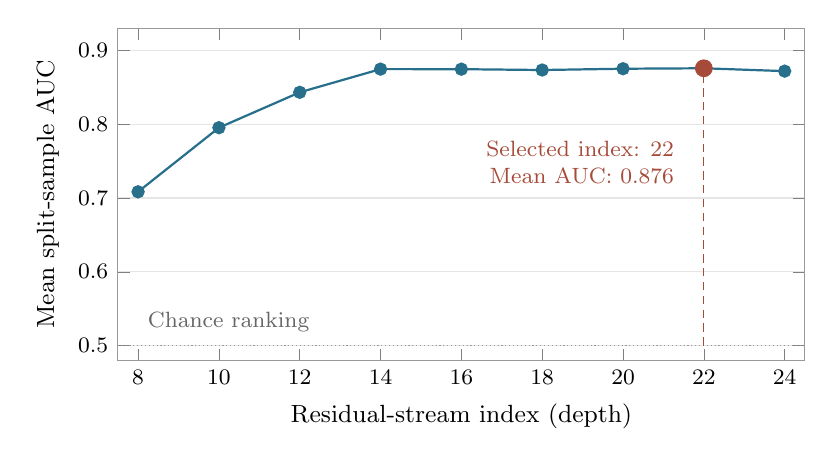
\begin{tikzpicture}
\definecolor{layerblue}{HTML}{286F8C}\definecolor{layerorange}{HTML}{A64B39}
\begin{axis}[width=.85\linewidth,height=5.8cm,xmin=7.5,xmax=24.5,ymin=.48,ymax=.93,xtick={8,10,12,14,16,18,20,22,24},ytick={.5,.6,.7,.8,.9},xlabel={Residual-stream index (depth)},ylabel={Mean split-sample AUC},label style={font=\small},tick label style={font=\footnotesize},axis line style={black!40},ymajorgrids,grid style={black!10}]
\addplot[black!40,densely dotted] coordinates {(7.5,.5)(24.5,.5)};
\addplot[thick,color=layerblue,mark=*,mark size=2pt] coordinates {(8,0.7083884479717814) (10,0.7952374790495909) (12,0.8431731790945042) (14,0.8745912616254232) (16,0.8745210846013124) (18,0.8733831898298773) (20,0.8751263186433994) (22,0.8757466150711491) (24,0.871869077743819)};
\draw[densely dashed,layerorange] (axis cs:22,.5) -- (axis cs:22,0.8757466150711491);
\addplot[only marks,mark=*,mark size=3pt,color=layerorange] coordinates {(22,0.8757466150711491)};
\node[font=\footnotesize,align=right,anchor=north east,text=layerorange] at (axis cs:21.5,.79) {Selected index: 22\\Mean AUC: 0.876};
\node[font=\footnotesize,anchor=south west,text=black!60] at (axis cs:8,.505) {Chance ranking};
\end{axis}\end{tikzpicture}
\par\medskip% The selected site feeds four exploratory questions; same samples are reused.
\begin{tikzpicture}[font=\fontsize{8.5}{10}\selectfont,
flow/.style={-{Latex[length=1.8mm]},thick,draw=black!45},
panel/.style={draw=black!20,rounded corners=2pt,fill=black!2,text width=3.0cm,align=center,inner sep=4pt,minimum height=2.4cm}]
\definecolor{pointblue}{HTML}{286F8C}
\definecolor{pointorange}{HTML}{A64B39}
\node[align=center,text width=13.6cm,font=\fontsize{10}{12}\selectfont\bfseries] (refit) at (7,0) {C. Re-estimate at index 22 on the full sample; examine MH1--MH4};
\coordinate (hub) at (7,-.55);
\draw[flow] (refit.south) -- (hub);
\node[panel,anchor=north] (one) at (1.7,-.95) {\textbf{MH\textsubscript{1}: signal}\\[3pt]Within-language AUC\\[4pt]\textcolor{pointblue}{All 21 cells above chance}};
\node[panel,anchor=north] (two) at (5.2,-.95) {\textbf{MH\textsubscript{2}: transfer}\\[3pt]Source A $\rightarrow$ target B\\[4pt]\textcolor{pointblue}{Reference and ANITA:\\higher transfer AUC}};
\node[panel,anchor=north] (three) at (8.7,-.95) {\textbf{MH\textsubscript{3}: behavior}\\[3pt]AUC / cosine\\vs. mean score\\[4pt]\textcolor{pointorange}{Mixed across models}};
\node[panel,anchor=north] (four) at (12.2,-.95) {\textbf{MH\textsubscript{4}: models}\\[3pt]Portability + addition\\[4pt]\textcolor{pointorange}{Portability differs\\Matched steering\\remains unresolved}};
\foreach \n in {one,two,three,four}{\draw[flow] (hub) -| (\n.north);}
\node[fit=(one)(two)(three)(four),inner sep=0] (checks) {};
\node[align=center,text width=13.6cm,text=black!65,font=\fontsize{8}{9.5}\selectfont] at ([yshift=-.5cm]checks.south) {Reused samples and shared question identities: these are exploratory checks, with no independent final question holdout.};
\end{tikzpicture}

\label{fig:mechanistic-layer-sweep}\fonte{Prepared by the author (2026).}\end{figure}


\paragraph*{MH\textsubscript{1}: is there an observable refusal-outcome contrast?} This check is necessary before asking whether a direction transfers or changes generation. At the selected index, the audit estimates one pooled direction per model using sampled outcomes from all seven languages, then calculates AUC separately within each language. Each cell asks whether that pooled axis distinguishes its refused and unsafe examples.

All 21 cells exceed chance ranking, with AUCs from $0.73$ to $1.00$ (Table~\ref{tab:mechanistic-refusal-projections}). This is consistent with MH\textsubscript{1}: even the more vulnerable AI Sweden model has an observable contrast. An unsafe model can carry such a signal because distinguishing two sampled outcomes does not imply that refusal dominates its ordinary behavior. These AUCs reuse rows that estimated the direction, so they describe in-sample separation rather than prediction on new questions. Each cell contains at most 24 examples per outcome; some safer-model cells have only 4--22 unsafe examples. A high AUC should therefore not obscure the small, outcome-selected sample.

\paragraph*{MH\textsubscript{2}: does that contrast carry across languages?} A high within-language AUC could reflect a language-specific distinction. To examine portability, the audit estimates a direction from one source language and projects outcomes in a different target language onto that fixed direction. For example, an Italian direction is assessed on Swedish examples without being re-estimated from those Swedish rows. The reverse test uses a Swedish direction on Italian examples and can differ. Seven languages yield $7\times6=42$ ordered pairs per model, or 126 across the three models.

Mean transfer AUC is $0.94$ for the reference and $0.93$ for ANITA, with all 42 pairs in each model above $0.7$. AI Sweden averages $0.69$, ranges from $0.40$ to $0.93$, and exceeds $0.7$ in 21 of 42 pairs. Values near one mean that a direction learned elsewhere still ranks refused outcomes above unsafe outcomes in the target language; a value below $0.5$ means the ranking tends to reverse for that transfer. The stronger, more uniform portability in the safer models is consistent with MH\textsubscript{2}. AI Sweden's variable results suggest a less stable cross-language contrast rather than complete absence of one. The $0.7$ comparison is descriptive, not a statistical-significance threshold.

All 126 source--target pairs share canonical prompt identities: 4--11 for AI Sweden, 5--17 for the reference, and 2--19 for ANITA. A transferred direction therefore crosses languages but is not assessed exclusively on unseen questions. This limits the result to language portability with possible prompt familiarity, rather than independent question generalization.

Figure~\ref{fig:mechanistic-separability-overview} makes the first two findings easier to compare. A blue circle describes separation under a pooled direction that has already used the plotted language's rows. An orange diamond instead averages directions learned in the six other languages and evaluated on that target language. The reference and ANITA retain high transfer separability in most targets, with a visible drop for Swahili. AI Sweden's transfer values are lower and more uneven. The figure compares descriptive diagnostics, not matched training and independent test performance.

\begin{figure}[p]\centering
\caption[Refusal-signal separability by language]{Refusal-signal separability at index 22. Blue circles use each model\textquotesingle s pooled direction on its estimation rows. Orange diamonds average the six directions learned in other languages and evaluated on the indicated target language. The dashed line is chance ranking ($0.5$). The summaries use different direction-estimation procedures; their gap is descriptive, not a held-out performance loss. All transfer pairs share some question identities.}

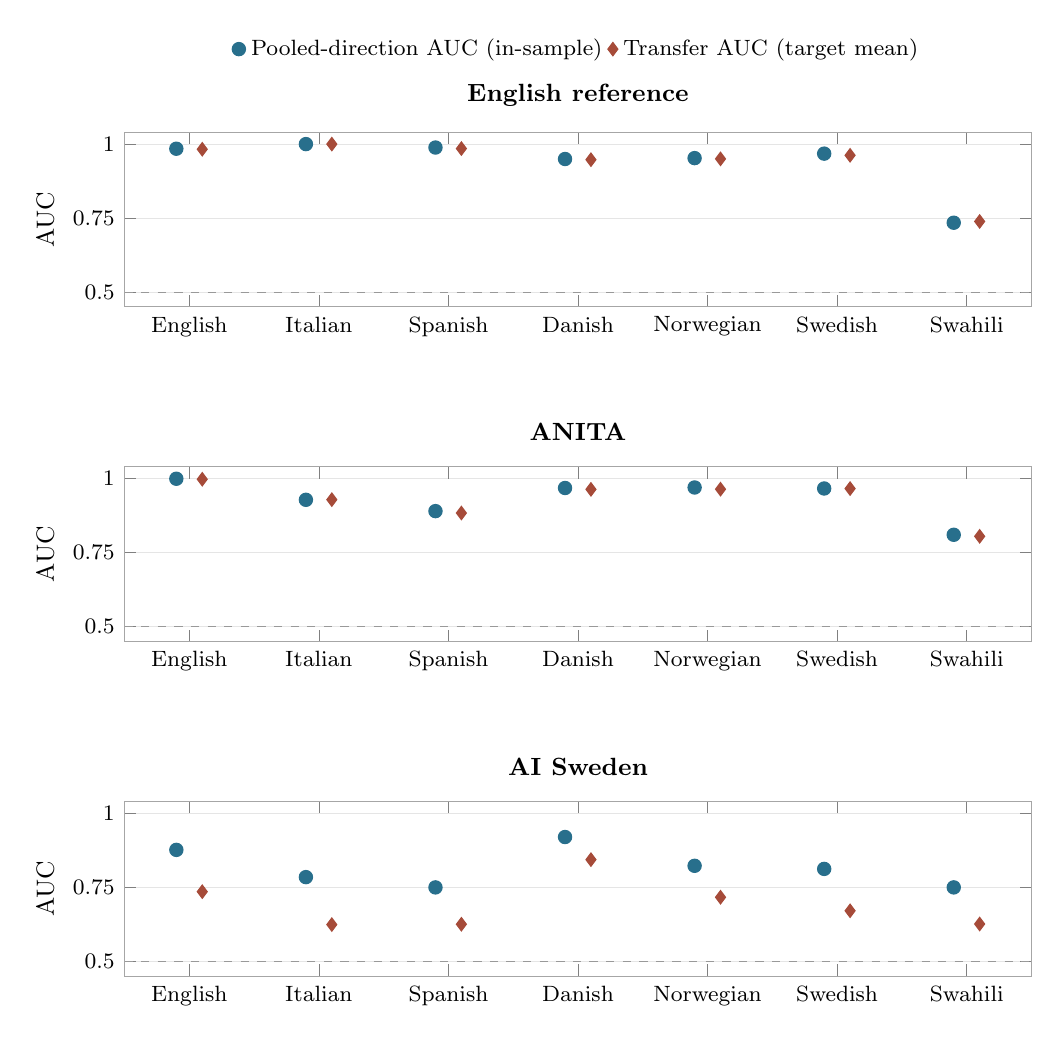
\begin{tikzpicture}
\definecolor{mechblue}{HTML}{286F8C}\definecolor{mechorange}{HTML}{A64B39}
\begin{axis}[width=13.1cm,height=3.8cm,at={(0,-0.0cm)},anchor=north west,xmin=-.5,xmax=6.5,ymin=.45,ymax=1.04,ytick={.5,.75,1},ylabel={AUC},xtick={0,1,2,3,4,5,6},xticklabels={English,Italian,Spanish,Danish,Norwegian,Swedish,Swahili},tick label style={font=\footnotesize},label style={font=\small},title={English reference},title style={font=\small\bfseries},axis line style={black!35},ymajorgrids,grid style={black!10},legend style={font=\footnotesize,draw=none,at={(.5,1.35)},anchor=south,legend columns=2}]
\addplot[black!40,dashed,forget plot] coordinates {(-.5,.5)(6.5,.5)};
\addplot[only marks,mark=*,mark size=2.4pt,color=mechblue] coordinates {(-0.1,0.984375000000) (0.9,1.000000000000) (1.9,0.988425925926) (2.9,0.949652777778) (3.9,0.952651515152) (4.9,0.967803030303) (5.9,0.734375000000)};
\addplot[only marks,mark=diamond*,mark size=2.4pt,color=mechorange] coordinates {(0.1,0.982638888889) (1.1,1.000000000000) (2.1,0.984953703704) (3.1,0.947337962963) (4.1,0.950126262626) (5.1,0.962121212121) (6.1,0.738715277778)};
\legend{Pooled-direction AUC (in-sample),Transfer AUC (target mean)}
\end{axis}
\begin{axis}[width=13.1cm,height=3.8cm,at={(0,-4.25cm)},anchor=north west,xmin=-.5,xmax=6.5,ymin=.45,ymax=1.04,ytick={.5,.75,1},ylabel={AUC},xtick={0,1,2,3,4,5,6},xticklabels={English,Italian,Spanish,Danish,Norwegian,Swedish,Swahili},tick label style={font=\footnotesize},label style={font=\small},title={ANITA},title style={font=\small\bfseries},axis line style={black!35},ymajorgrids,grid style={black!10},legend style={font=\footnotesize,draw=none,at={(.5,1.35)},anchor=south,legend columns=2}]
\addplot[black!40,dashed,forget plot] coordinates {(-.5,.5)(6.5,.5)};
\addplot[only marks,mark=*,mark size=2.4pt,color=mechblue] coordinates {(-0.1,1.000000000000) (0.9,0.928819444444) (1.9,0.890625000000) (2.9,0.968750000000) (3.9,0.970486111111) (4.9,0.967105263158) (5.9,0.810763888889)};
\addplot[only marks,mark=diamond*,mark size=2.4pt,color=mechorange] coordinates {(0.1,0.998263888889) (1.1,0.929398148148) (2.1,0.884259259259) (3.1,0.964120370370) (4.1,0.964699074074) (5.1,0.966739766082) (6.1,0.805555555556)};
\end{axis}
\begin{axis}[width=13.1cm,height=3.8cm,at={(0,-8.5cm)},anchor=north west,xmin=-.5,xmax=6.5,ymin=.45,ymax=1.04,ytick={.5,.75,1},ylabel={AUC},xtick={0,1,2,3,4,5,6},xticklabels={English,Italian,Spanish,Danish,Norwegian,Swedish,Swahili},tick label style={font=\footnotesize},label style={font=\small},title={AI Sweden},title style={font=\small\bfseries},axis line style={black!35},ymajorgrids,grid style={black!10},legend style={font=\footnotesize,draw=none,at={(.5,1.35)},anchor=south,legend columns=2}]
\addplot[black!40,dashed,forget plot] coordinates {(-.5,.5)(6.5,.5)};
\addplot[only marks,mark=*,mark size=2.4pt,color=mechblue] coordinates {(-0.1,0.876736111111) (0.9,0.784722222222) (1.9,0.750000000000) (2.9,0.920138888889) (3.9,0.822916666667) (4.9,0.812500000000) (5.9,0.750000000000)};
\addplot[only marks,mark=diamond*,mark size=2.4pt,color=mechorange] coordinates {(0.1,0.735532407407) (1.1,0.624421296296) (2.1,0.625578703704) (3.1,0.843750000000) (4.1,0.716724537037) (5.1,0.671006944444) (6.1,0.626446759259)};
\end{axis}
\end{tikzpicture}
\label{fig:mechanistic-separability-overview}
\fonte{Prepared by the author (2026).}
\end{figure}

\FloatBarrier

\paragraph*{MH\textsubscript{3}: does clearer separation coincide with less harmful assistance?} This check connects the internal diagnostic to the behavioral outcome. Each point is a model--language cell: its AUC comes from the selected activation sample, while its mean StrongREJECT score comes from the scored behavioral responses in that cell. Spearman's $\rho$ compares the rankings of these summaries. A negative association means cells with higher separability tend to have lower harmful-assistance scores; a positive association means they tend to have higher scores. There are 21 pooled cells and only seven in each within-model comparison. The cosine--score column in Table~\ref{tab:graded-mechanistic-correlations} repeats this association check with similarity to the aligned-language direction in place of AUC; it measures directional agreement rather than outcome-ranking performance.

The pooled association is negative ($\rho=\GMechPooledRho{}$), and both the reference and ANITA have within-model $\rho=-0.86$. AI Sweden instead has a positive association ($\rho=\GMechSwedenRho{}$; Table~\ref{tab:graded-mechanistic-correlations}). For a concrete contrast, its Danish cell has AUC $0.920$ and mean score $0.490$, whereas its Swahili cell has AUC $0.750$ and mean score $0.029$. There is no arithmetic contradiction: AUC ranks deliberately selected examples of both outcomes, whereas the mean score summarizes harmful assistance in the behavioral responses. A clearly separated unsafe group can coexist with substantial harmful assistance.

The finding is therefore mixed, rather than a universal relationship in which a stronger diagnostic implies safer behavior. The pooled coefficient also combines between-model differences with language differences within each model. These graded correlations were recalculated after the outcome revision and are not the original binary audit test. Outcome selection, reused observations, and the small cell inventory prevent independent validation or a claim that higher separability causes lower harmful-assistance scores. Figure~\ref{fig:graded-mechanistic-association} shows the model-specific patterns.

\GradedMechanisticCorrelationTable

\FloatBarrier
\Needspace{12\baselineskip}
\paragraph*{MH\textsubscript{4}: what does the ANITA--AI Sweden contrast establish?} The preceding checks describe each model's signal and its associations. This expectation asks whether the safer derivative combines a more stable cross-language direction with a stronger refusal-associated response to intervention. Cosine and transfer address different parts: cosine compares direction orientations within a model, whereas transfer AUC tests whether a source direction ranks target-language outcomes. A cosine near one means similar orientation; near zero means little directional agreement. Directions from different checkpoints are not compared component by component in one shared coordinate system.

ANITA's non-aligned-language directions have cosines of $0.69$--$0.90$ with its Italian anchor, and its mean transfer AUC is $0.93$, compared with AI Sweden's $0.69$. Its raw difference-in-means vector is also larger ($4.93$ versus $2.53$), but this norm is sensitive to each model's activation scale and is measured before normalization. It must not be read as ANITA having roughly twice as much safety alignment. Orientation and transfer provide the clearer evidence of a more portable sampled contrast.

Addition asks whether moving activations along the estimated direction has behavioral consequences during generation, beyond an association in recorded vectors. The following figure and table report graded scores after addition at the inspected strengths. Different, post-hoc strengths and reused prompt samples prevent establishing which model is more steerable under a matched intervention. MH\textsubscript{4} therefore has descriptive support for the portability contrast, while comparative steerability and a causal explanation remain unresolved. Different starting checkpoints and adaptation histories also prevent identifying one training stage as the cause.

\setcounter{secnumdepth}{3}

\clearpage
Figure~\ref{fig:mechanistic-intervention-scores} visualizes the graded scores after adding the direction; Table~\ref{tab:mechanistic-intervention} retains the exact sample accounting. Each point describes the selected intervention sample at its reported strength. There is no matched zero-strength rerun against which to interpret these as measured score reductions.

\begin{figure}[htbp]\centering
\caption[Graded scores after refusal-direction addition]{Mean graded scores after addition at the reported, post-hoc strengths. The denominator shown beside each point is scored responses out of generated responses; two AI Sweden responses are unscored. These are reused, outcome-selected prompts at different strengths, with no zero-strength rerun or independent controls. A low score can also reflect irrelevant or degenerate output; it is not by itself evidence of successful refusal.}

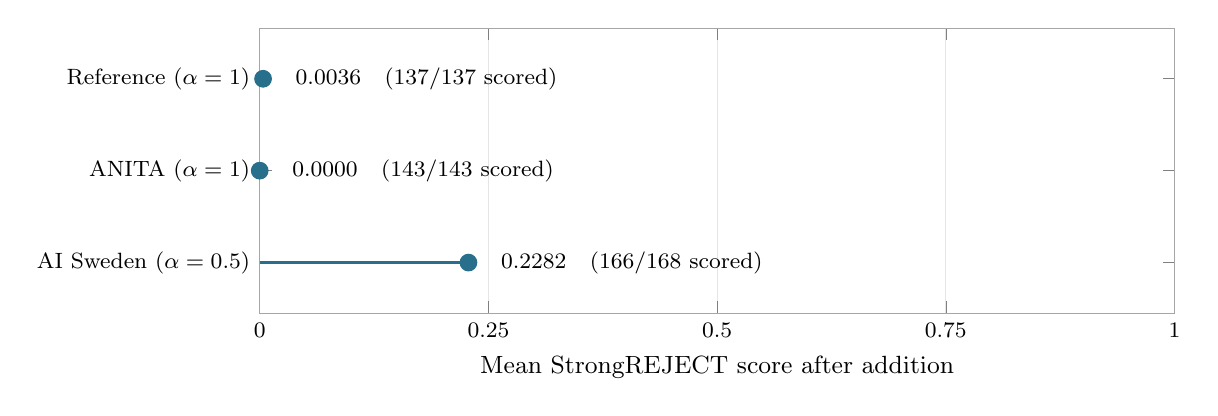
\begin{tikzpicture}
\definecolor{mechblue}{HTML}{286F8C}\definecolor{mechorange}{HTML}{A64B39}
\begin{axis}[width=13.2cm,height=5.2cm,xmin=0,xmax=1,ymin=-.55,ymax=2.55,ytick={0,1,2},yticklabels={AI Sweden ($\alpha=0.5$),ANITA ($\alpha=1$),Reference ($\alpha=1$)},xlabel={Mean StrongREJECT score after addition},xtick={0,.25,.5,.75,1},tick label style={font=\footnotesize},label style={font=\small},axis line style={black!35},xmajorgrids,grid style={black!10},clip=false]
\addplot[mechblue,thick,forget plot] coordinates {(0,2)(0.003649635036,2)};
\addplot[only marks,mark=*,mark size=3pt,mechblue,forget plot] coordinates {(0.003649635036,2)};
\node[anchor=west,font=\footnotesize] at (axis cs:0.028649635036,2) {0.0036\quad(137/137 scored)};
\addplot[mechblue,thick,forget plot] coordinates {(0,1)(0.000000000000,1)};
\addplot[only marks,mark=*,mark size=3pt,mechblue,forget plot] coordinates {(0.000000000000,1)};
\node[anchor=west,font=\footnotesize] at (axis cs:0.025000000000,1) {0.0000\quad(143/143 scored)};
\addplot[mechblue,thick,forget plot] coordinates {(0,0)(0.228162650602,0)};
\addplot[only marks,mark=*,mark size=3pt,mechblue,forget plot] coordinates {(0.228162650602,0)};
\node[anchor=west,font=\footnotesize] at (axis cs:0.253162650602,0) {0.2282\quad(166/168 scored)};
\end{axis}
\end{tikzpicture}
\label{fig:mechanistic-intervention-scores}
\fonte{Prepared by the author (2026).}
\end{figure}

\GradedInterventionTable
\defensenote{What the intervention establishes}{Adding the estimated direction changes generation, so the vector is behaviorally consequential on these prompts. It does not prove that the vector is the unique refusal mechanism or that post-training caused the between-model difference. The missing independent prompts, alpha-zero rerun, random direction, and norm-matched control are the reason to say ``consistent with a functional refusal direction'' rather than ``causally identifies the mechanism.''}

The addition intervention applies $+\alpha\hat{r}$ at residual layer 22 during prompt and generation passes, scaled by the model's mean residual norm. Table~\ref{tab:mechanistic-intervention} reports the mean saved StrongREJECT scores at the inspected strengths, with unscored responses shown separately. The response sample was selected by historical outcomes and reused for direction estimation. These are conditional score summaries after perturbation, not population jailbreak rates or controlled causal treatment effects.

This intervention does not by itself identify a unique refusal mechanism. No $\alpha=0$ reproducibility run, random-direction control, norm-matched control direction, or independent prompt holdout was included. Consequently, the between-model contrast could partly reflect general sensitivity to residual perturbation, and effect sizes may be optimistic because direction estimation and intervention reuse the same prompt sample. At higher strengths, manual inspection found repetitive or degenerate text; $\alpha=2$ is therefore a failure regime, not evidence of successful refusal. The reportable strengths ($\alpha=1$ for the reference and ANITA, $\alpha=0.5$ for AI Sweden) were chosen post hoc after inspecting degeneration and should be treated as diagnostics rather than comparable dose optima. A zero graded score can mean refusal, irrelevant output, or degeneration; low scores alone do not establish restored safety behavior.

More generally, diagnostic separability alone is insufficient to identify what a representation causally encodes. \textcite{hewittDesigningInterpretingProbes2019} show why probing results require control tasks or baselines that distinguish information present in a representation from structure learned or exploited by the probe. The present difference-in-means probe is deliberately simple, but the missing random-direction, held-out, and matched harmless controls remain relevant for exactly this reason.

\subsection{Mechanism Decision Matrix}
\label{sec:mechanism-decision-matrix}

Table~\ref{tab:mechanistic-decision-matrix} summarizes the evidence against the four exploratory expectations. The most defensible interpretation is narrower than a complete mechanism: the safer derivative exhibits a more cross-lingually portable refusal-outcome contrast, while the vulnerable derivative exhibits a weaker and more heterogeneous one. The data do not show that post-training literally shortened or erased a unique refusal representation, nor do they separate harm recognition from refusal execution. They therefore offer a plausible internal correlate of the model-specific behavioral pattern, not a causal decomposition of how that pattern arose.

\begin{table}[htbp]
\centering
\scriptsize
\caption[Evidence matrix for the refusal-direction audit]{Evidence matrix for the exploratory audit. Representation expectations preceded extraction; the graded behavioral association was revised afterwards. No external preregistration is claimed.}
\label{tab:mechanistic-decision-matrix}
\begin{tabular}{@{}p{0.06\linewidth}p{0.30\linewidth}p{0.44\linewidth}p{0.10\linewidth}@{}}
\toprule
ID & Test & Outcome & Verdict \\
\midrule
MH\textsubscript{1} & Within-language projection AUC above $0.5$ & All 21 in-sample cells $0.73$--$1.00$; layer-selection split score $0.876$ & Consistent \\
MH\textsubscript{2} & Cross-lingual transfer AUC (train-A, eval-B) & Reference $0.94$, ANITA $0.93$ (all pairs $>0.7$); AI Sweden $0.69$ (half below) & Consistent \\
MH\textsubscript{3} & Per-cell separability versus mean score & Revised pooled $\rho=\GMechPooledRho{}$; AI Sweden $\rho=\GMechSwedenRho{}$ & Mixed \\
MH\textsubscript{4} & Model contrast: portability and steerability & Portability differs; matched steerability remains untested & Partial \\
\bottomrule
\end{tabular}
\fonte{Prepared by the author (2026).}
\end{table}

The direction-similarity heatmap (Figure~\ref{fig:mechanistic-direction-similarity}), the full transfer matrices (Figure~\ref{fig:mechanistic-transfer-matrices}), the separability-versus-score scatter (Figure~\ref{fig:graded-mechanistic-association}), the layer sweep (Figure~\ref{fig:mechanistic-layer-sweep}) and the two supporting tables (Tables~\ref{tab:mechanistic-refusal-projections} and~\ref{tab:mechanistic-language-direction-similarity}) are generated directly from the published audit artifacts. Figures~\ref{fig:residual-stream}, \ref{fig:mechanistic-methodology}, and~\ref{fig:mechanistic-direction-construction} are explanatory schematics; the other figures plot saved audit measurements. The separability overview and intervention-score plot summarize these measurements close to their interpretation.

\MechTransferAnalysisText

\paragraph*{Connecting the reference's behavioral and mechanistic profiles.} The English reference's language profile in Section~\ref{sec:reference-baseline-results} has a corresponding exploratory mechanistic observation. Among its thirteen behavioral language cells, Swahili has the lowest BELEBELE specialization and the highest mean StrongREJECT score (Figures~\ref{fig:strongreject-profiles}--\ref{fig:belebele-profiles}). The transfer audit shows that Swahili is also a comparatively difficult target for refusal-outcome directions learned in other languages (Figure~\ref{fig:mechanistic-transfer-matrices}), even though the reference's transfer is strong overall and a direction learned in Swahili transfers well elsewhere. Thus, the result concerns reduced separability in Swahili under transferred directions, rather than the absence of a portable direction learned from Swahili.

Read together, these observations connect three distinct measurements: benign comprehension and answer consistency, separation of refused versus complied harmful prompts in activation space, and the harmful assistance present in generated responses. They are compatible with language capability and the cross-language portability of refusal-associated representations jointly helping to interpret the reference's behavior. They do not establish a causal pathway from lower SPEC to weaker refusal or higher harmful-assistance scores. The mechanistic audit covers seven languages and uses outcome-selected harmful prompts; it does not measure harmful-versus-harmless recognition. Source and target evaluations overlap in prompt identity, and independent question holdouts and intervention controls remain incomplete. This is therefore an exploratory internal correlate of the descriptive reference pattern, not independent validation of H\textsubscript{1} or H\textsubscript{2}.

\defensebox{How to read the transfer matrices}{Rows identify the source language used to estimate the direction; columns identify the target language being evaluated. Swahili can supply a portable direction while remaining a difficult target. All directed transfer pairs share some canonical prompt identities, so this is transfer across languages with possible prompt familiarity, not an independent question holdout. Also distinguish the layer-selection split from final testing: its test halves were reused to select among nine layers.}

\MechDirectionSimilarityFigure
\MechTransferMatrixFigure
\begin{figure}[htbp]\centering
\caption[Refusal-signal diagnostics and graded scores]{Saved refusal-signal diagnostics versus mean graded score. Language cells are descriptive and outcome-selected activation samples are not independent held-out evaluations.}

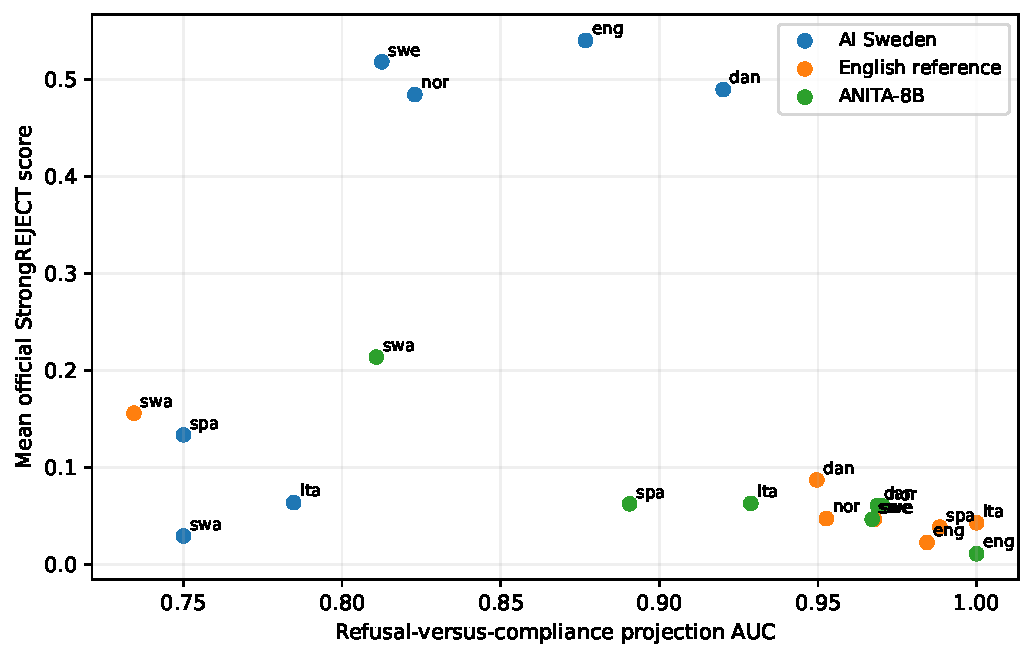
\includegraphics[width=.9\linewidth]{figures/graded_mechanistic_association.pdf}
\label{fig:graded-mechanistic-association}\fonte{Prepared by the author (2026).}\end{figure}
\GradedMechanisticCellsTable
\MechLanguageDirectionSimilarityTable

\FloatBarrier

\end{otherlanguage*}
